\documentclass[12pt]{report}
\usepackage[utf8]{inputenc}
\usepackage[T1]{fontenc}
\usepackage[francais]{babel}
\usepackage{listings}
\usepackage{xcolor}
\usepackage{csquotes}
\usepackage{float} % Grace a ce package, je peux mettre H dans les position des images pour le placer ICI
\usepackage[backend=bibtex, bibencoding=ascii, sorting=nty]{biblatex} %Pour utiliser biblatex
\bibliography{mabib.bib} %Syntax for version < 1.2

\usepackage{pdfpages} % Pour inclure des pdf dans le document
\makeindex
\setcounter{tocdepth}{3} % Profondeur de la table of content
\setcounter{secnumdepth}{3} % Jusqu'où sera affiché le sectionning
% Valeurs par défaut le lstset
\lstset{
	language=C,	
	frame=single, 
	numbers=left,
	rulecolor=\color{black},
	backgroundcolor=\color{lightgray},
	literate= {á}{{\'a}}1 {é}{{\'e}}1 {í}{{\'i}}1 {ó}{{\'o}}1 {ú}{{\'u}}1
  			  {Á}{{\'A}}1 {É}{{\'E}}1 {Í}{{\'I}}1 {Ó}{{\'O}}1 {Ú}{{\'U}}1
  			  {à}{{\`a}}1 {è}{{\`e}}1 {ì}{{\`i}}1 {ò}{{\`o}}1 {ù}{{\`u}}1
  			  {À}{{\`A}}1 {È}{{\'E}}1 {Ì}{{\`I}}1 {Ò}{{\`O}}1 {Ù}{{\`U}}1
  			  {ä}{{\"a}}1 {ë}{{\"e}}1 {ï}{{\"i}}1 {ö}{{\"o}}1 {ü}{{\"u}}1
  			  {Ä}{{\"A}}1 {Ë}{{\"E}}1 {Ï}{{\"I}}1 {Ö}{{\"O}}1 {Ü}{{\"U}}1
  			  {â}{{\^a}}1 {ê}{{\^e}}1 {î}{{\^i}}1 {ô}{{\^o}}1 {û}{{\^u}}1
  			  {Â}{{\^A}}1 {Ê}{{\^E}}1 {Î}{{\^I}}1 {Ô}{{\^O}}1 {Û}{{\^U}}1
  			  {œ}{{\oe}}1 {Œ}{{\OE}}1 {æ}{{\ae}}1 {Æ}{{\AE}}1 {ß}{{\ss}}1
  			  {ç}{{\c c}}1 {Ç}{{\c C}}1 {ø}{{\o}}1 {å}{{\r a}}1 {Å}{{\r A}}1
  			  {€}{{\EUR}}1 {£}{{\pounds}}1,
   	commentstyle=\scriptsize\ttfamily\slshape, % style des commentaires
	basicstyle=\scriptsize\ttfamily, % style par défaut
   	keywordstyle=\scriptsize\rmfamily\bfseries,% style des mots-clés
   	frame=trbl,% Style du cadre
	inputencoding=utf8, 
	showspaces=false, 
	showstringspaces=false, 
	tabsize=2, % sets default tabsize to 2 spaces
   	escapechar=°}  % Caractère d'échappement, permet des commandes latex dans la source
% -----------------------------------------------------
\begin{document}
\includepdf[pages={1}]{garde/page_de_garde.pdf}
\chapter*{Remerciements}

\paragraph{}
Je tiens à remercier l’ESI qui m’a permis de trouver ce stage chez Toyota ainsi que M. Alain Coquelet pour m’avoir accepté en tant que stagiaire au sein de l’entreprise.
\paragraph{}
Je remercie également toute l’équipe qui m’a accueilli, aidé et avec qui j'ai passé de bons moments tout le long de ce stage. 

\tableofcontents

\chapter{Summary}

\paragraph{}
TOYOTA Belgium is the entreprise where I was internship.
There was several big projects to develop and M. Coquelet chose me to do the Showroom Visit application (a Proof of Concept). 

\paragraph{}
During some events like the Auto Show or any showroom visit, there is a lot of visitors that come to discover the brand. Those people are very important.

The application will be used to help the sellers to show which vehicles correspond to the wishes of the visitor. 
It will also be used to save some informations about the visitor (like his e-mail adress or phone number) to contact him after the event if he is in a hurry and must leave. 

\paragraph{}
I had to develop it in ASP .NET MVC5 with HTML5, CSS3, JavaScript and C\# languages. I used SQL Server to access to the databases. I never developped in ASP .NET but I had two weeks to learn this technology and it was enough. 

\paragraph{}
Finally, I have finished it in time but I did not implement some features because it stays a Proof Of Concept. 
This is not the main purpose of a POC to develop the application entirely.

\chapter{Introduction}

\paragraph{}
TOYOTA Belgium est l'entreprise dans laquelle j'ai travaillé ces quatre derniers mois.
Son but est de fournir des véhicules Toyota/Lexus, créer des évènements (par exemple, journée porte ouverte) et faire de la publicité pour la marque.

\paragraph{}
Le but de mon stage était de développer une application Web (pour tablette) permettant d'aider les vendeurs lors d'évènements tels que les visites showroom. L'une des principales fonctionnalités de cette application était d'afficher tous les types de véhicules correspondant aux désirs du visiteur tout en captant les coordonnées de celui-ci. 
 
\paragraph{}
Pour ce faire, la technologie choisie par mes chefs de projet fut l'ASP .NET MVC5 avec les langages HTML5, CSS3, JavaScript et C\#. Quant à la gestion des bases de données, le SGBD utilisé est Microsoft SQL Server. Je ne l'avais jamais utilisé mais il s'est avéré être facile à appréhender.

\paragraph{}
Concernant la gestion du projet, il fallait créer un planning sous Excel incluant ma charge de travail estimée et réelle pour chacune des parties que compose l’application ainsi que tout autre évènement influant le stage tel que notre pré-présentation de stage. 

\paragraph{}
La méthode de travail utilisée était itérative; il m’avait été demandé initialement de coder certaines parties de l’application, à la suite de quoi une réunion organisée avec mes chefs de projet permettait de mettre en avant les éléments à supprimer, changer ou encore les fonctionnalités à rajouter.

\paragraph{}
Au bout de ces quatre mois, l'application est terminée, il manque cependant quelques fonctionnalités qui n'ont pas été développées car le projet n'était qu'un Proof Of Concept et non une application destinée à être utilisée.

\chapter{Présentation générale}
La présentation générale se divisera en trois grandes parties : 

\begin{itemize}
\item La première présentera l'entreprise.
\item La seconde se chargera de décrire l'environnement de travail.
\item Quant à la troisième, il s'agira d'une présentation de mon application.
\end{itemize}

\section{Présentation de l'entreprise}
La présentation de l'entreprise va se diviser en deux parties. La première se chargera d'expliquer qu'est-ce que TOYOTA et la seconde décrira l'entreprise où j'ai personnellement travaillé.
\subsection*{TOYOTA en général}

\paragraph{}
Toyota Motor Corporation est une multinationale dans le domaine de l'automobile, créée par Kiichiro Toyoda en 1933 et est basée au Japon.
Avec le temps, l'entreprise est devenue 1$^{er}$ constructeur automobile mondial en 2012 avec un chiffre d’affaires de 265,7 milliards de dollars.

\paragraph{}
L'entreprise possède également une filiale en Europe qui s'occupe des principaux pays européens tel que la France et l'Allemagne. La Belgiqe n'est pas concernée par Toyota Europe. 

\subsection*{TOYOTA Belgium}
\paragraph{}
TOYOTA Belgium n'est pas une filiale de TOYOTA Europe mais plutôt d'Inchcape (Entreprise Londonienne possédant tout un réseau de garages).

\paragraph{}
Elle fournit des véhicules Toyota/Lexus, organise des évènements spéciaux mais aussi de la publicité pour la marque. Elle possède environ 120 employés là où j'ai travaillé (Zaventem). 

\paragraph{}
L'entreprise possède également environ 4\% des parts du marché en Belgique, mais elle rencontre beaucoup plus de succès en dehors de l'Europe (TOYOTA est le leader mondial de l'automobile).


\section{Présentation de l'environnement}
\paragraph{}
J'ai développé mon application dans le département IT de TOYOTA Belgium avec un ordinateur portable fourni par l'entreprise. Un DELL dont le processeur est un Intel Core i5 cadencé à 2,60 GHz, 4 Go de RAM, écran Full HD, etc. 
En résumé, un ordinateur très puissant qui n'a jamais eu de soucis à faire tourner mon programme ni n'importe quel autre.

\paragraph{}
Au niveau applicatif, j'ai eu droit à une adresse e-mail (\textit{xxx.yyy@toyota.be}) qui était le moyen officiel de créer des réunions et envoyer des e-mails. 
J'ai aussi eu droit à la suite Office (Word, Excel, PowerPoint, etc.), un accès VPN au réseau intranet de l'entreprise ainsi que l'environnement de développement intégré "Visual Studio" sur lequel j'ai développé mon application.

\section{Présentation de l'application}
La présentation de l'application se déroulera en plusieurs étapes : tout d'abord, une mise en contexte suivi du but de l'application, les technologies utilisées pour la réalisation de l'application et enfin, la présentation de l'application en soi.

\subsection{Contexte}
\paragraph{}
Lors d'évènements tels que les journées portes ouvertes, les salons de l'auto, ou simplement lors de visites showroom, de nombreuses personnes viennent pour découvrir la marque. 
Il serait dès lors très avantageux de capter les intérêts de ces personnes en vue de les satisfaire au cas par cas en leur apportant de plus amples informations sur les modèles de la gamme correspondant le plus à leurs besoins.

\paragraph{}
En outre, Il serait également intéressant de pouvoir obtenir certaines coordonnées telles que l'adresse e-mail ou le  numéro de téléphone du visiteur au cas où celui-ci serait pressé et voudrait être recontacté ultérieurement.

\paragraph{}
L'application que je développerai devra donc être destinée aux tablettes pour ainsi permettre au vendeur d'aller vers le visiteur et lui montrer tout ce qui correspond à ses intérêts.

\subsection{But}
\paragraph{}
Le but de l'application est bien évidemment de vendre davantage de voitures TOYOTA. Dans un pays comme la Belgique où la concurrence est telle que de nombreuses marques de voitures se disputent les parts du marché, n'importe quelle opportunité est à prendre au sérieux. Idéalement, le but de l'application serait d'augmenter le nombre de ventes d'au moins 1 par mois et par concessionnaire.

\subsection{Les bénéficiaires}
\paragraph{}
L'application est destinée à être utilisée par les vendeurs présent sur les stand lors d'évènements tels que des journées portes ouvertes, le salon de l'auto ou les visites showroom.

\subsection{Technologies utilisées}
\paragraph{}
L'application devait être développée en ASP .NET MVC5 et les langages étaient l'HTML5, le CSS3, le JavaScript (côté client) et le C\# (côté serveur). La raison de vouloir faire une application Web plutôt qu'une "vraie" est le désir rendre celle-ci multi-OS en évitant ainsi la multiplication du code en développant l'application sur Android, iOS et Windows.

\subsection{Méthodologie de travail}
\paragraph{}
Il m'a été demandé de tenir un planning sous Excel retraçant l'ensemble de mes activités, la charge de travail estimée de celles-ci ainsi que leur charge de travail réelle.
Cela permettait notamment de savoir où j'en étais dans l'avancement du projet par rapport au temps dont je disposais, savoir si je devais accélérer le rythme ou pas.

\paragraph{}
La méthode de travail utilisée était itérative; il m’avait été demandé initialement de coder certaines parties de l’application, à la suite de quoi une réunion organisée avec mes chefs de projet permettait de mettre en exergue les éléments à supprimer, modifier ou encore les fonctionnalités à rajouter.

\paragraph{}
Cette procédure de travail constitue un réel avantage car elle permet d’avoir un retour immédiat des utilisateurs  laissant notamment la possibilité de modifier l’application en fonction de leur convenance. 

\subsection{L'application}
\paragraph{}
L'application se divise en trois parties :

\begin{itemize}
\item La fenêtre Home
\item La fenêtre Product Specification
\item La fenêtre Customer
\end{itemize}

\subsubsection*{Home}
\paragraph{}
Après authentification, il s'agit du point d'entrée de l'application, c'est dans cette fenêtre que sont affichés toutes les visites en cours. Elles pourront être sauvegardées, effacées, en créer et sauter de l'une à l'autre instantanément.
(voir ci-dessous, figure \ref{image_home})

\begin{figure}[H]
	\caption{Fenêtre d'accueil de l'application}
	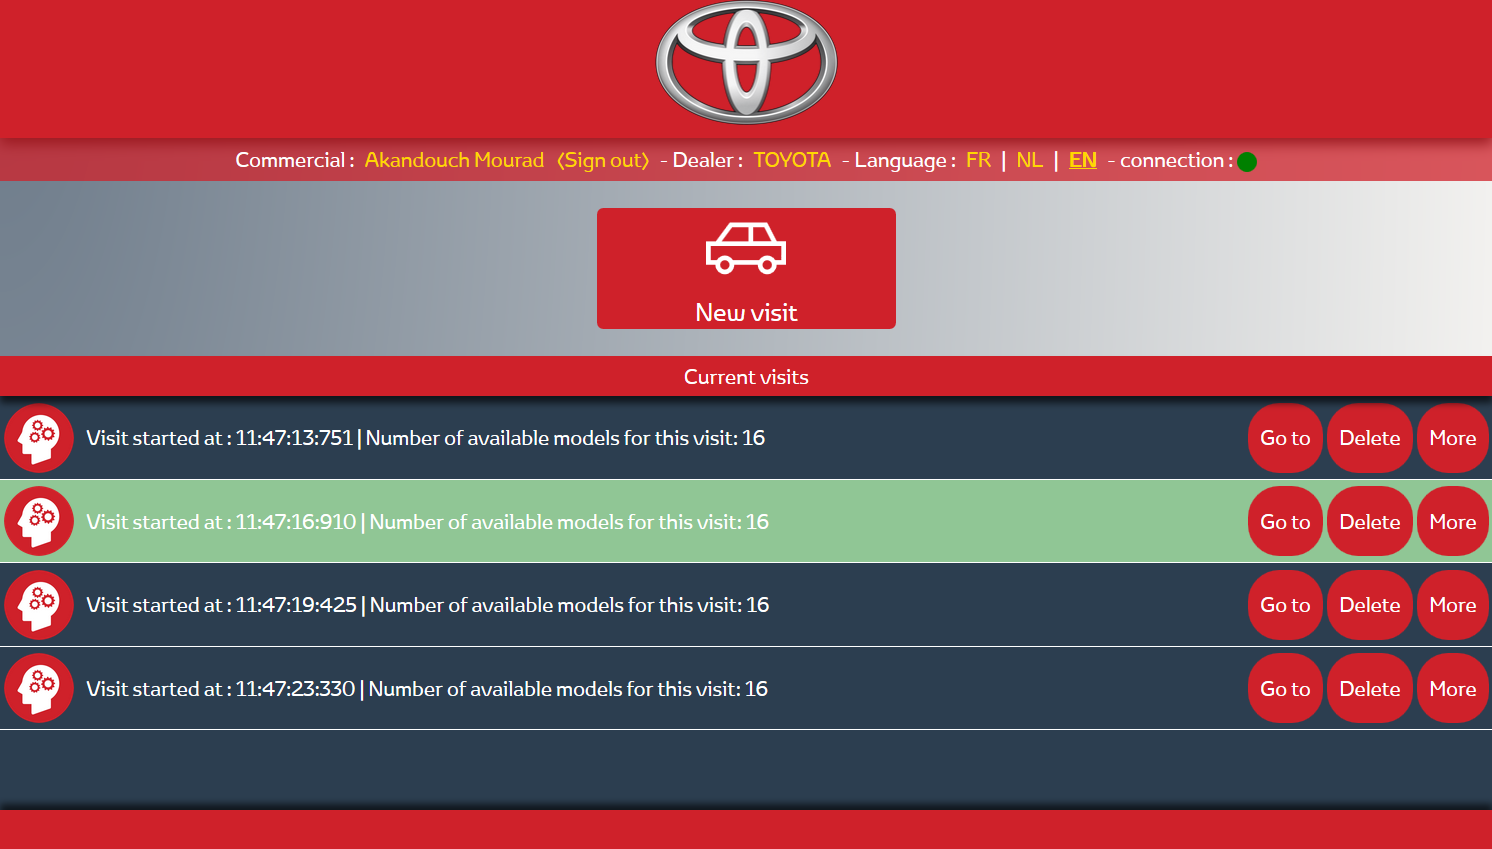
\includegraphics[width=\linewidth]{img/image_home}
	\label{image_home}
\end{figure}

\paragraph{}
À terme, il était également prévu que l'application puisse fonctionner en mode déconnecté s'il arrivait qu'une panne de réseau se produise. Le programme ne se connecterait non plus aux bases de données de TOYOTA mais à une cache sauvegardée localement au démarrage de l'application (nécessite donc au moins une connexion au démarrage).
\paragraph{}
Cette fonctionnalité n'a pas pu être réalisée par manque de temps, nous pouvons cependant voir un indicateur de l'état du réseau dans la barre de statut.
\paragraph{}
Cette fenêtre affiche également une barre de statut dans laquelle sont affichés des informations concernant le vendeur authentifié. Des informations telles que le nom, le prénom et le concessionnaire auquel appartient le vendeur. 
Le choix de la langue d'affichage de l'application y figure aussi.

\subsubsection*{Product Specification}
\paragraph{}
Fenêtre principale de l'application, celle-ci permet de définir les intérêts du visiteur. Elle est divisée en plusieurs sous-fenêtres dont : 

\begin{itemize}
\paragraph{}
\item Une permettant de définir les intérêts les plus courants chez les visiteurs. Il s'agit ici des critères les plus probables d'apparaître lors d'une discussion entre le vendeur et le visiteur. Par exemple, le budget du visiteur ou la (les) catégorie(s) qui l'intéresse telle(s) qu'une voiture compacte, une SUV, voiture de ville, une utilitaire, etc.

\begin{figure}[H]
	\caption {
	Critères principaux revenant souvent lors d'une visite, nous pouvons notamment y voir : Le modèle (AYGO, YARIS, 
	VERSO, etc.), la catégorie (SUV, Ville, Utilitaire, etc.), le type de carburant (Hybride, diesel, essence, etc.), 
	le type de transmission (manuelle, automatique, multidrive, etc.), le nombre de roues motrices, le budget, la 
	cylindrée en cm$^{3}$, la puissance du véhicule, le nombre de portes et enfin le nombre de places.
	}
	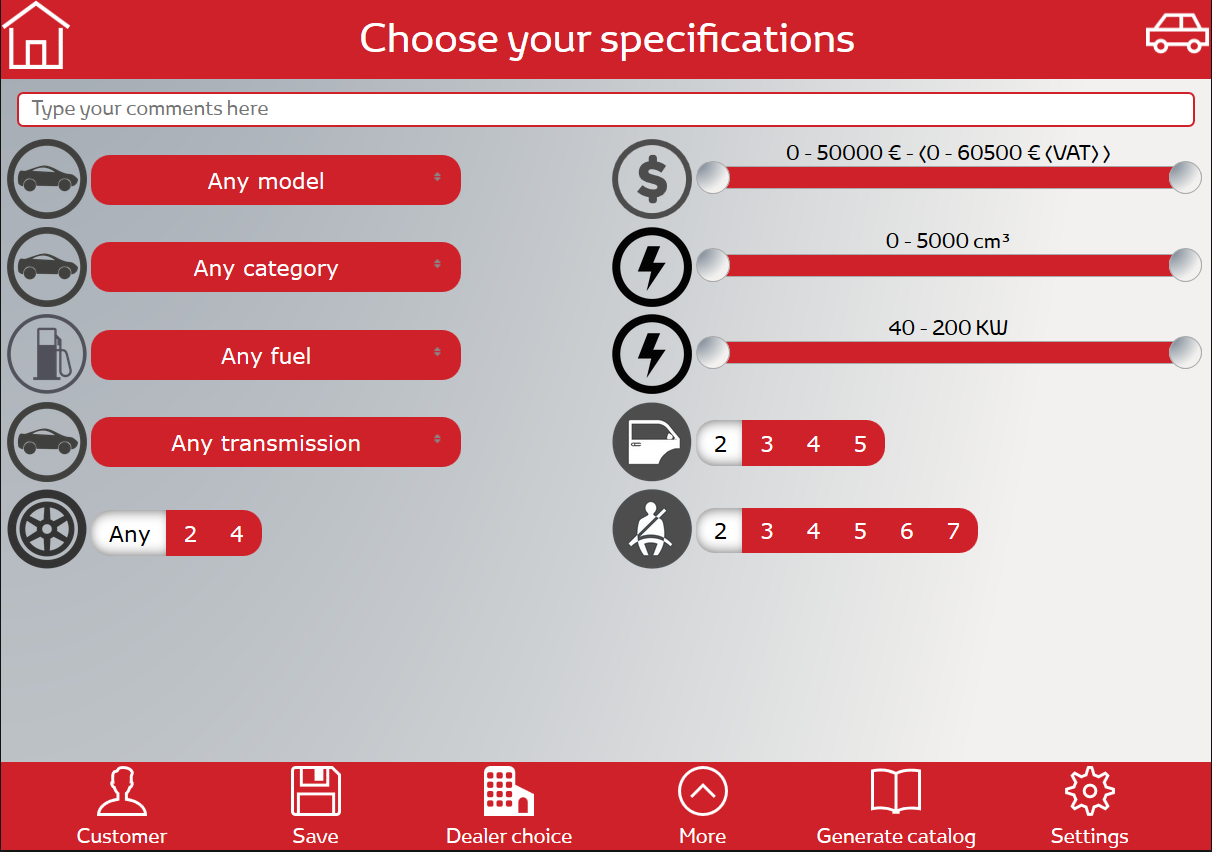
\includegraphics[width=\linewidth]{img/image_product_1}
	\label{image_product_1}
\end{figure}

\item Une seconde permettant de définir des critères moins courants tels que ceux liés à la fiscalité (Avantage toute nature, Taxe de mise en circulation, etc.). 
Supposons que le visiteur disposerait d'un garage, cela l'amènerait probablement à ne rechercher que certains types de véhicules aux dimensions telles que la voiture y rentrerait sans encombre. Des filtres sur les dimensions sont donc également disponibles.

\begin{figure}[H]
	\caption {
	Critères secondaires revenant moins souvent lors d'une visite.
	Cette fenêtre s'ouvre grâce au bouton "More" et se ferme de la même manière.
	Nous pouvons y voir des critères tels que l'Avantage Toute Nature, la Taxe de Mise en Circulation, la consommation 
	de CO$_{2}$ au gramme par kilomètre, le nombre de chevaux fiscaux, les dimensions (longueur, largeur, hauteur), le 
	volume du coffre et le poids tractable par le véhicule. Ces critères ne sont pas définitifs, ils sont évidemment 
	encore à discuter avec l'utilisateur final de l'application.
	}
	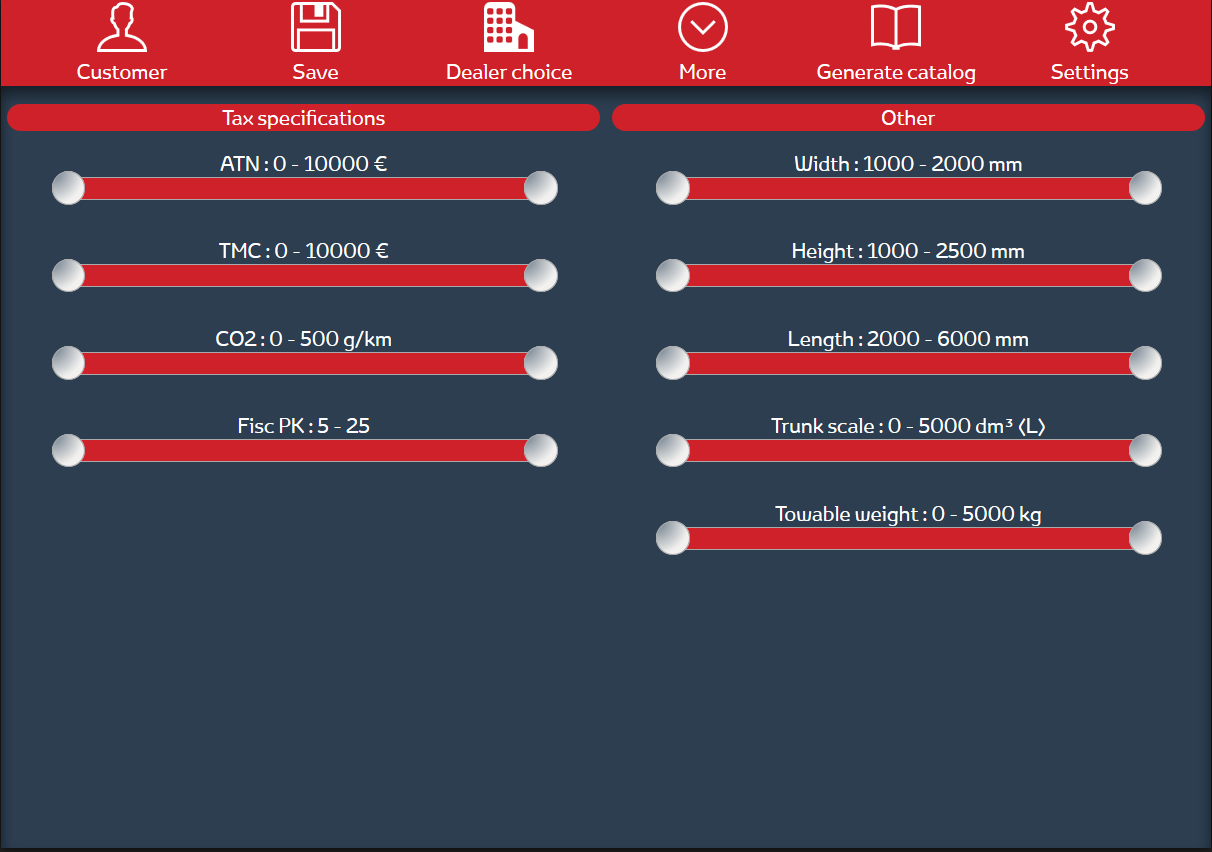
\includegraphics[width=\linewidth]{img/image_product_2}
	\label{image_product_2}
\end{figure}

\item Afin de consulter quels sont les modèles disponibles dans la gamme en fonction des critères choisis, il suffit d'appuyer sur le bouton en forme de voiture dans le coin supérieur droit de la fenêtre à la figure \ref{image_product_1}. Une nouvelle sous-fenêtre s'affichera alors avec la liste des modèles disponibles (voir ci-dessous, figure \ref{image_product_3}).

À terme, pour chacun des véhicules, il sera possible d'afficher des informations sur celle-ci, ses spécifications techniques, les équipements/couleurs disponibles, les taxes liées ainsi que ses USP's.\footnote{ "USP est l’acronyme pour Unique Selling Proposition ou argument clé de vente. L’USP est la promesse principale utilisée dans le cadre d’un discours publicitaire ou d’un entretien de vente. Pour délivrer tout son potentiel de conviction, l’USP (unique selling proposition) ne doit pas pouvoir être utilisée par la concurrence et doit être basée sur un élément réellement différenciateur. Le principe de l’USP a été développé et popularisé par Rosser Reeves." - \cite{DefinitionUSP} }

\begin{figure}[H]
	\caption{Ensemble des modèles disponibles correspondant aux critères désirés}
	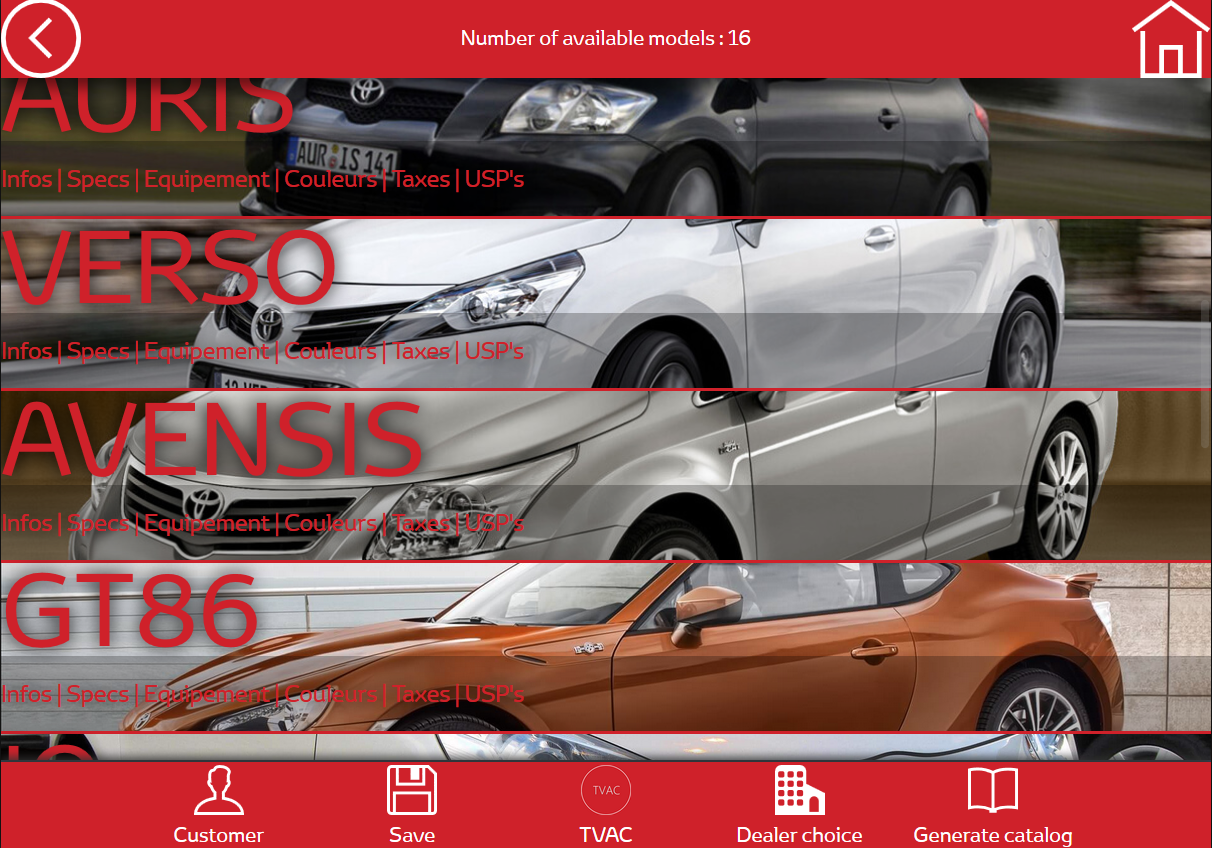
\includegraphics[width=\linewidth]{img/image_product_3}
	\label{image_product_3}
\end{figure}


\item Enfin, une dernière permet d'afficher le détail de chaque véhicule correspondant à un modèle précis.
Pour l'ouvrir, il suffit d'appuyer n'importe quel modèle.
(voir ci-dessous, figure \ref{image_product_4}).

\begin{figure}[H]
	\caption{Détail des véhicules disponibles pour la VERSO-S, nous pouvons remarquer qu'il existe une remise sur 
	certains types de VERSEO-S.
	Les remises sont caractérisées par un prix barré suivi d'une réduction en couleur or.
	D'autres informations pertinentes apparaissent comme le grade du véhicule, son prix, son numéro de série (aussi 
	appelé Code T-BEL), etc.}
	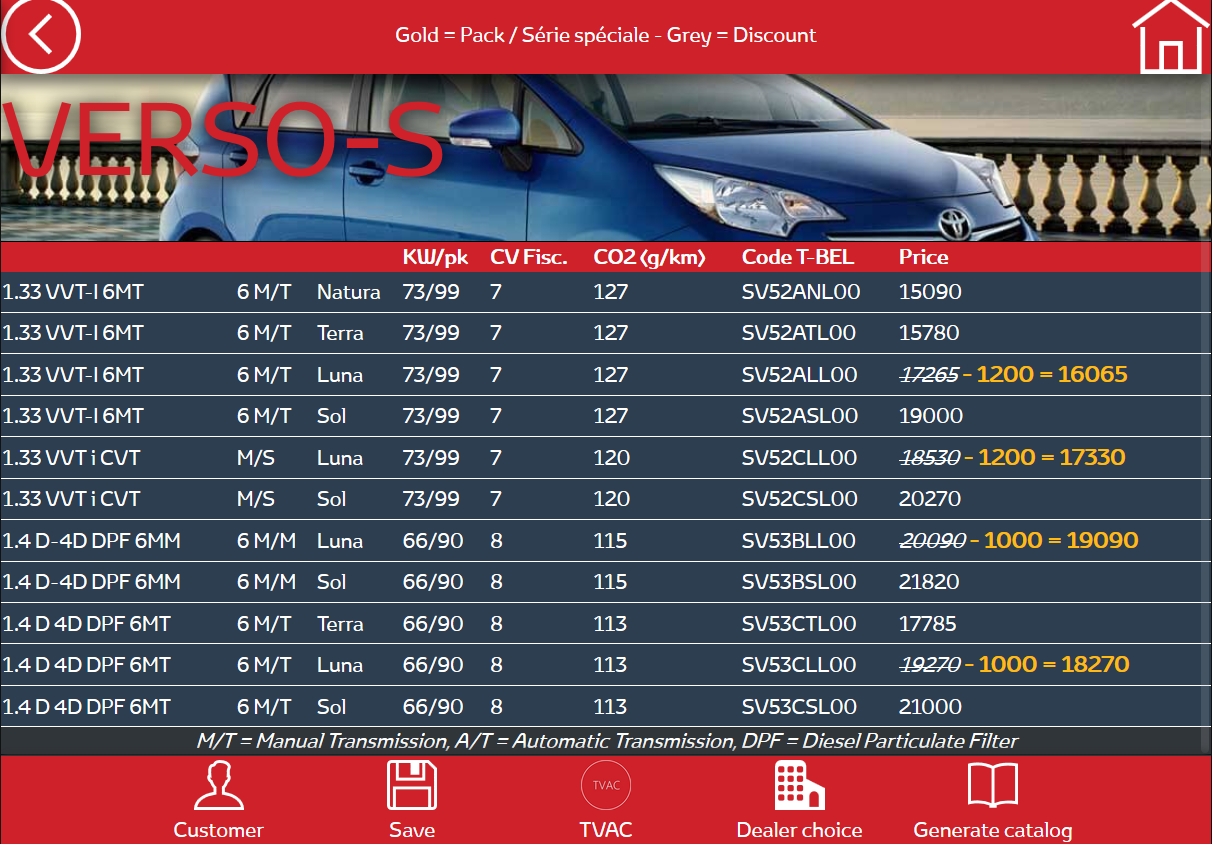
\includegraphics[width=\linewidth]{img/image_product_4}
	\label{image_product_4}
\end{figure}

\end{itemize}

\subsubsection*{Customer}
\paragraph{}
Troisième et dernière fenêtre de l'application, elle est essentielle pour la prise de coordonnées à la volée.
Il arrive aussi que certaines personnes viennent juste pour s'informer en ne laissant aucune coordonnée. Dans la plupart des cas, ce genre de visite ne sera pas enregistré (Ci-dessous, figure \ref{image_customer_3}).

\begin{figure}[H]
	\caption{Accueil de la fenêtre Customer}
	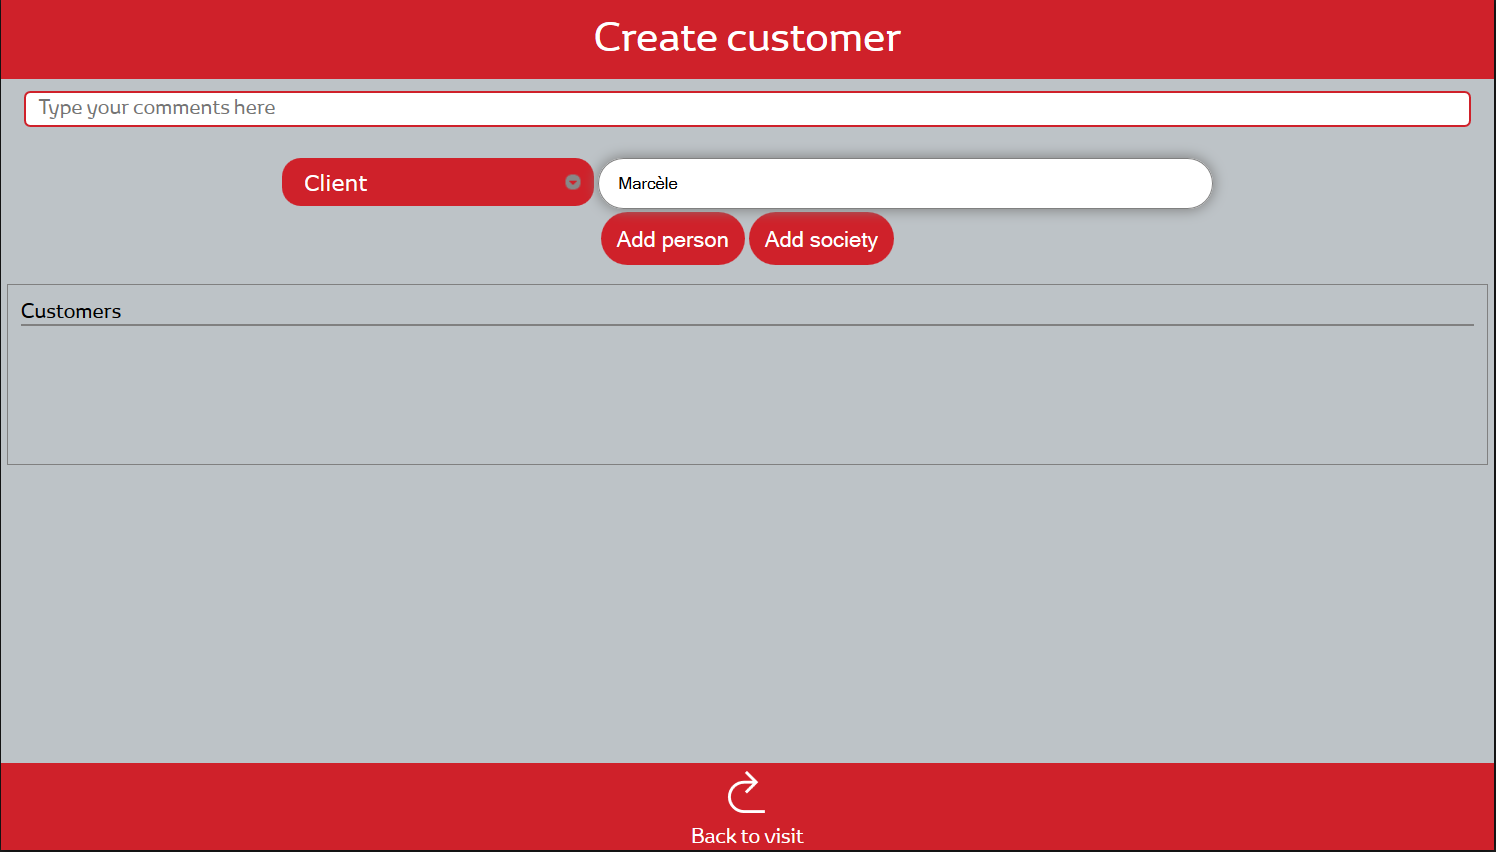
\includegraphics[width=\linewidth]{img/image_customer_3}
	\label{image_customer_3}
\end{figure}

\paragraph{}
Pour insérer un nouveau client dans cette fenêtre, il faut taper le nom du visiteur (ou de l'entreprise qu'il représente s'il vient en tant que contact société) et toucher le bouton "Add person"/"Add Society".
\paragraph{}
Il faut aussi savoir que les champs disponibles diffèrent en fonction du type de visiteur (contact société, personne, etc.).
Ci-dessous, les champs apparaissant lors de l'ajout d'une personne et d'une entreprise.

\begin{figure}[H]
	\caption{Champs correspondants à un visiteur simple.}
	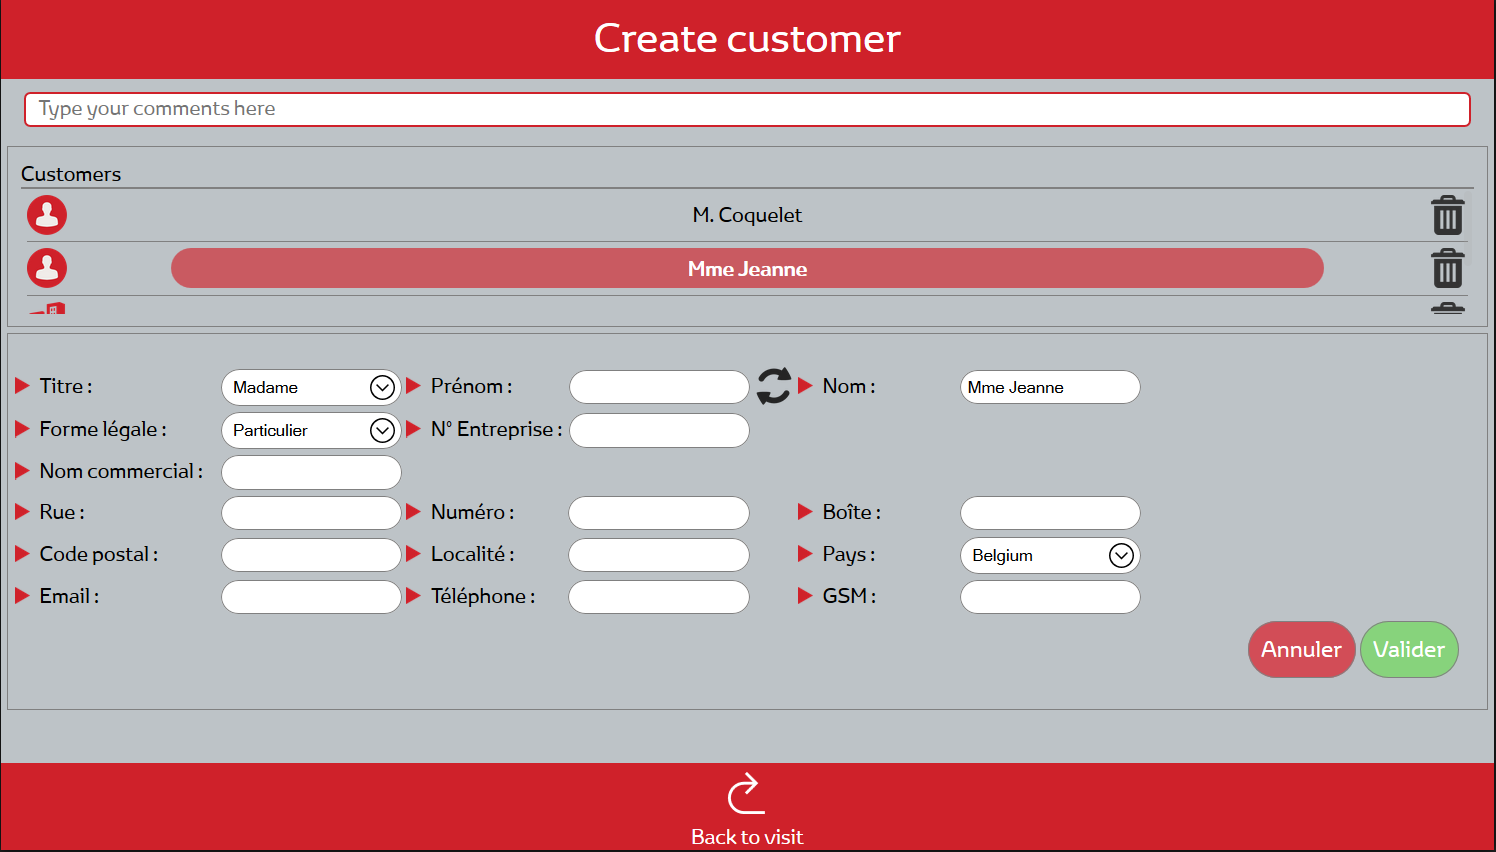
\includegraphics[width=\linewidth]{img/image_customer_1}
	\label{image_customer_1}
\end{figure}

\begin{figure}[H]
	\caption{Champs correspondants à une société.}
	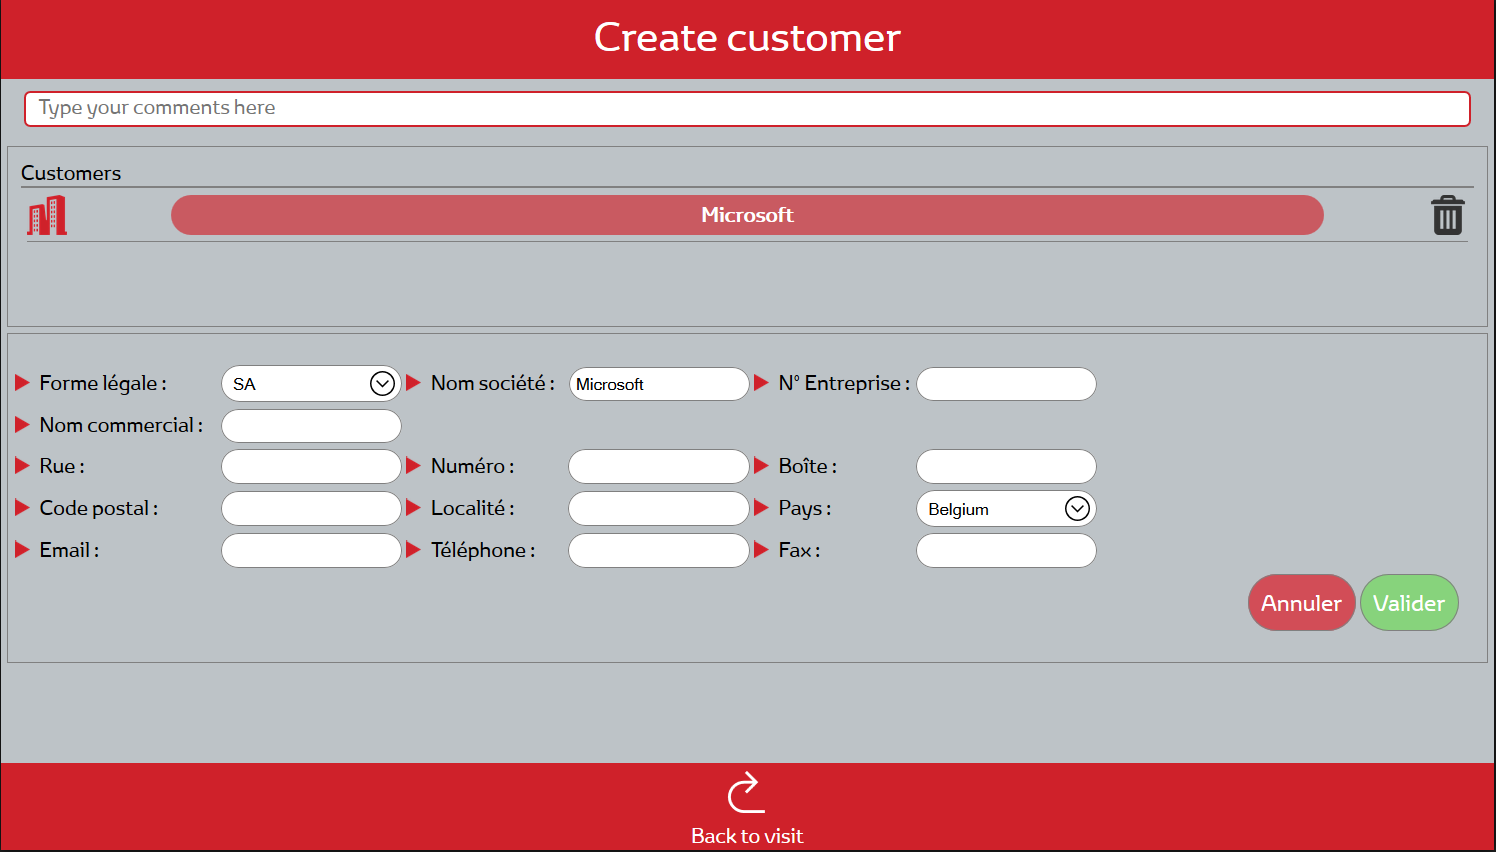
\includegraphics[width=\linewidth]{img/image_customer_2}
	\label{image_customer_2}
\end{figure}

\chapter{Carnet de bord}
Ci-dessous, un carnet de bord reprenant un bref résumé de chacune de mes semaines passées chez TOYOTA.
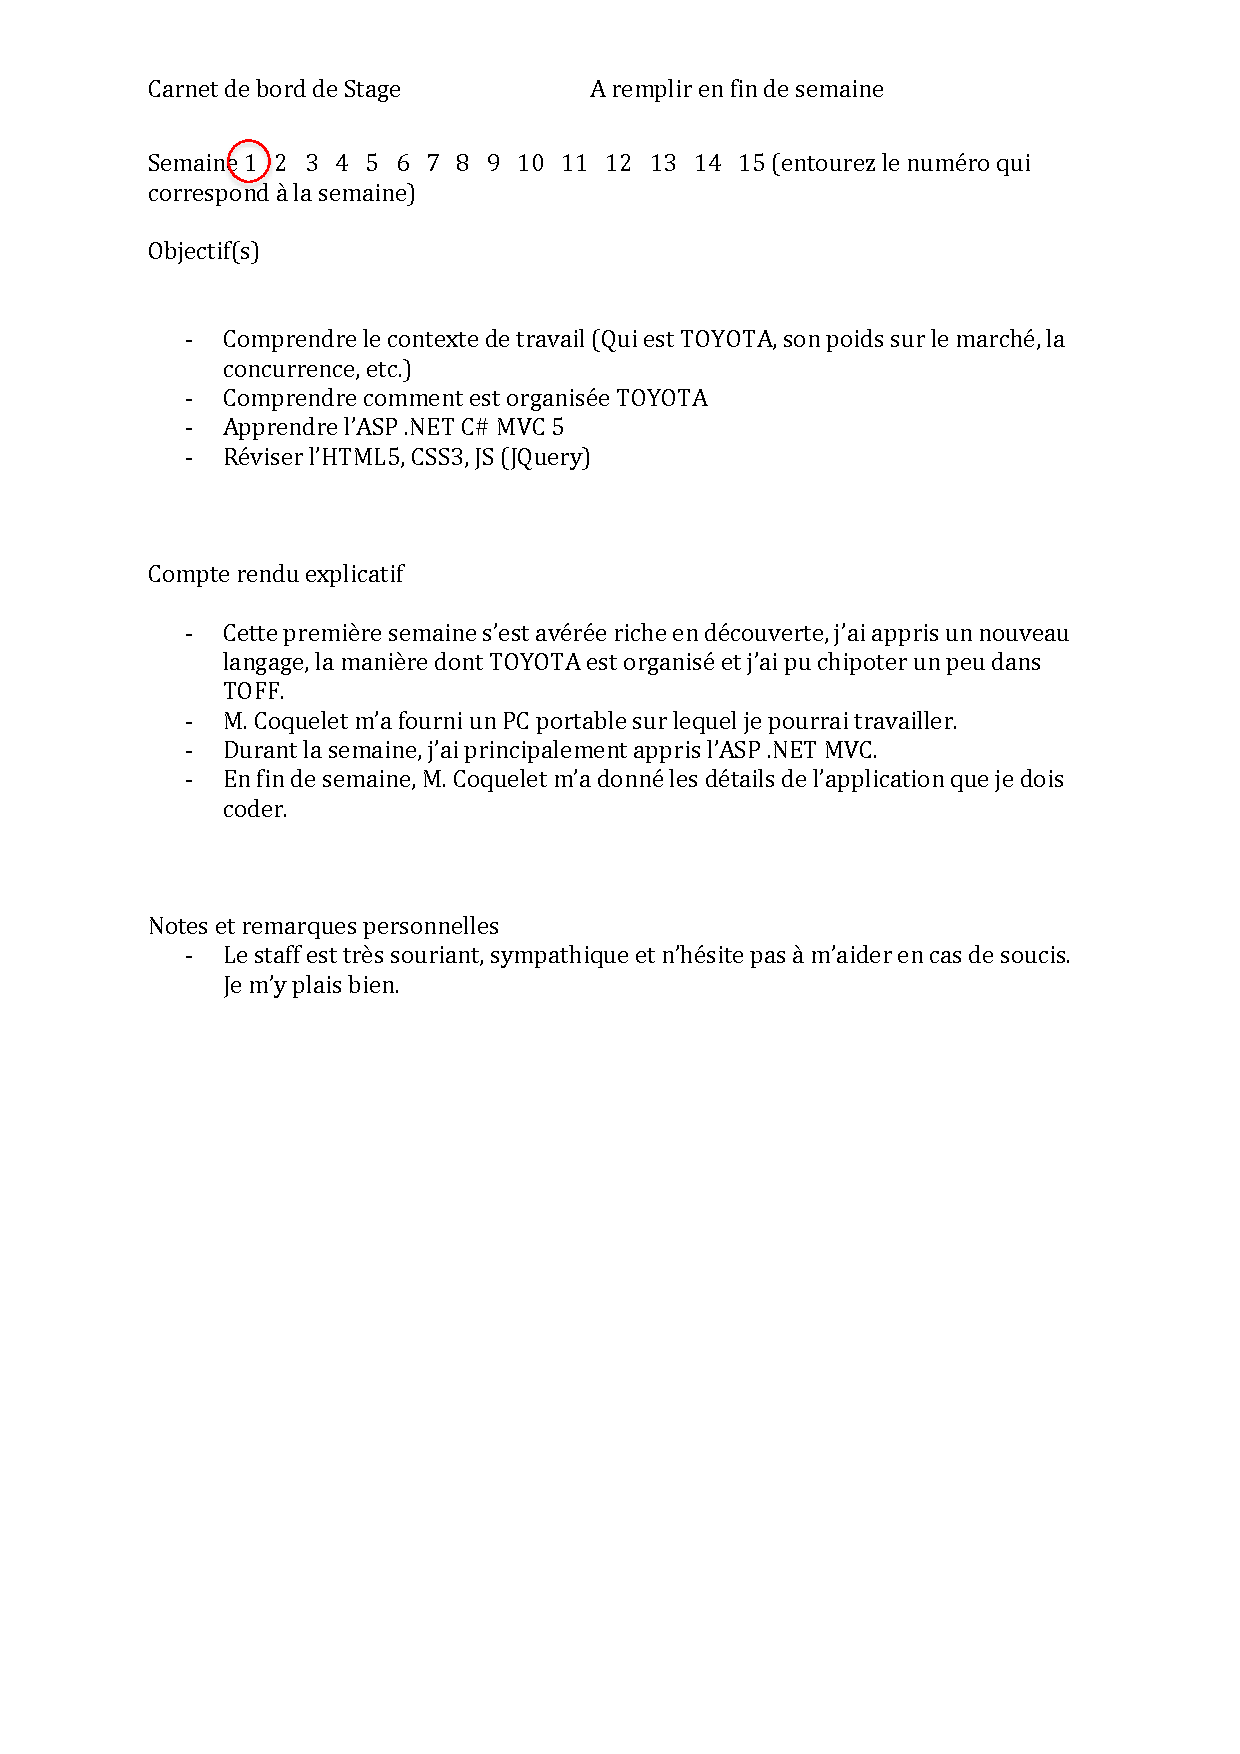
\includepdf[pages={1}]{carnets/Carnet_de_bord_de_Stage_S1.pdf}
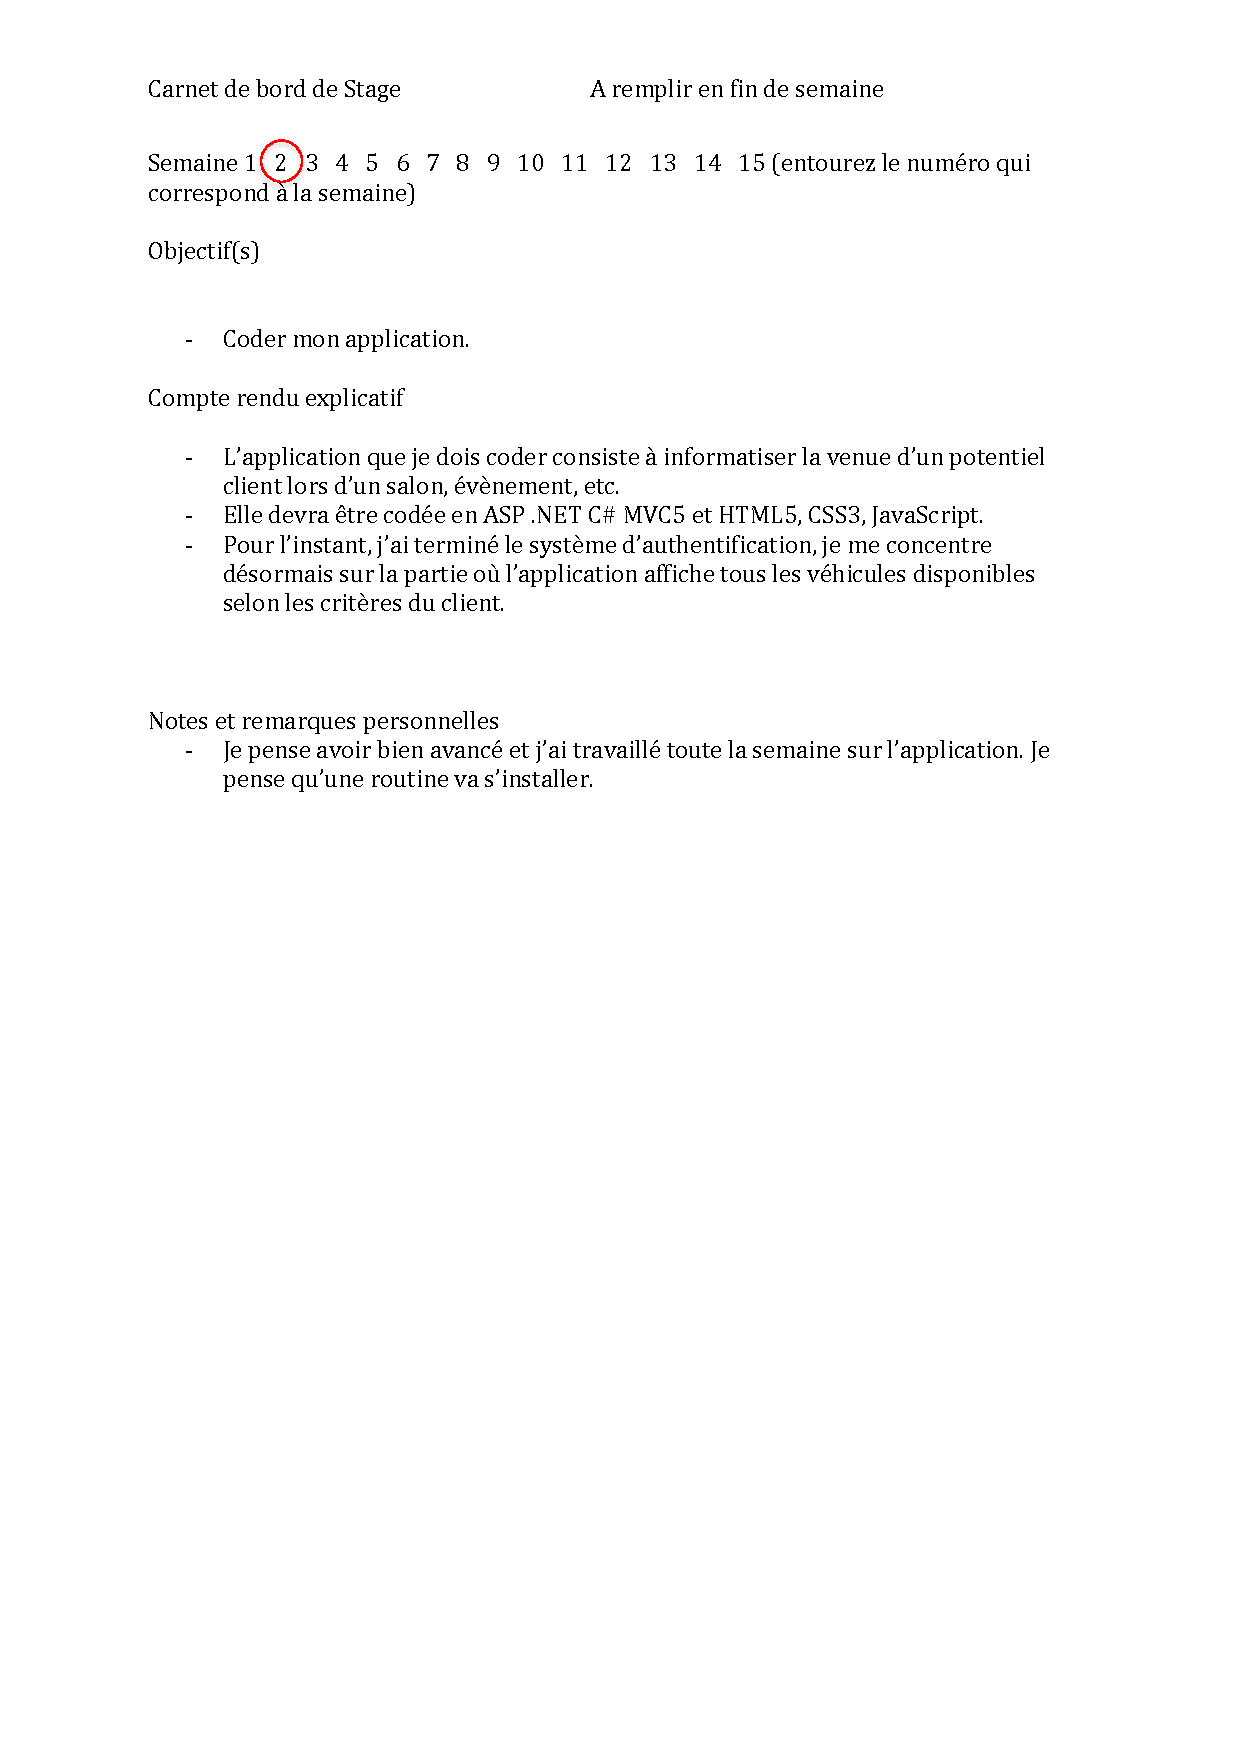
\includepdf[pages={1}]{carnets/Carnet_de_bord_de_Stage_S2.pdf}
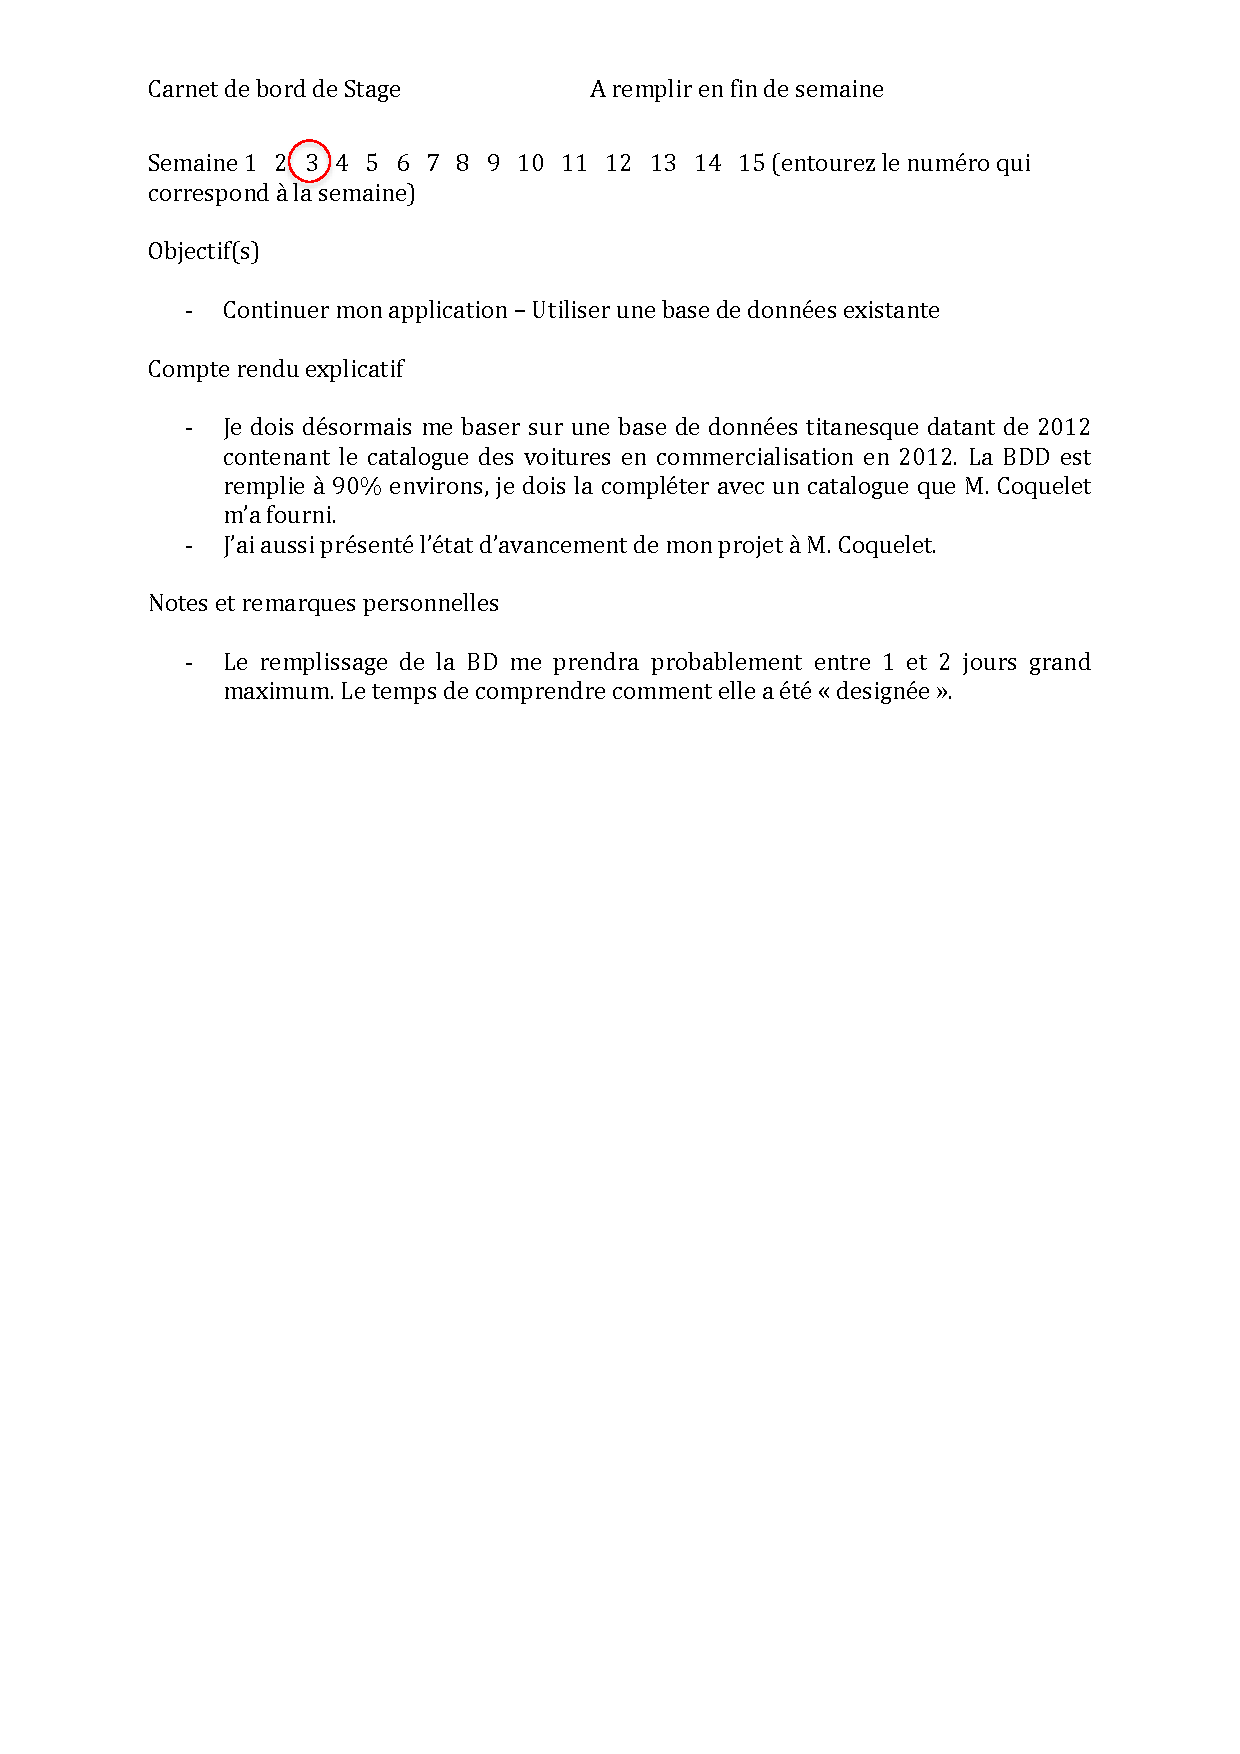
\includepdf[pages={1}]{carnets/Carnet_de_bord_de_Stage_S3.pdf}
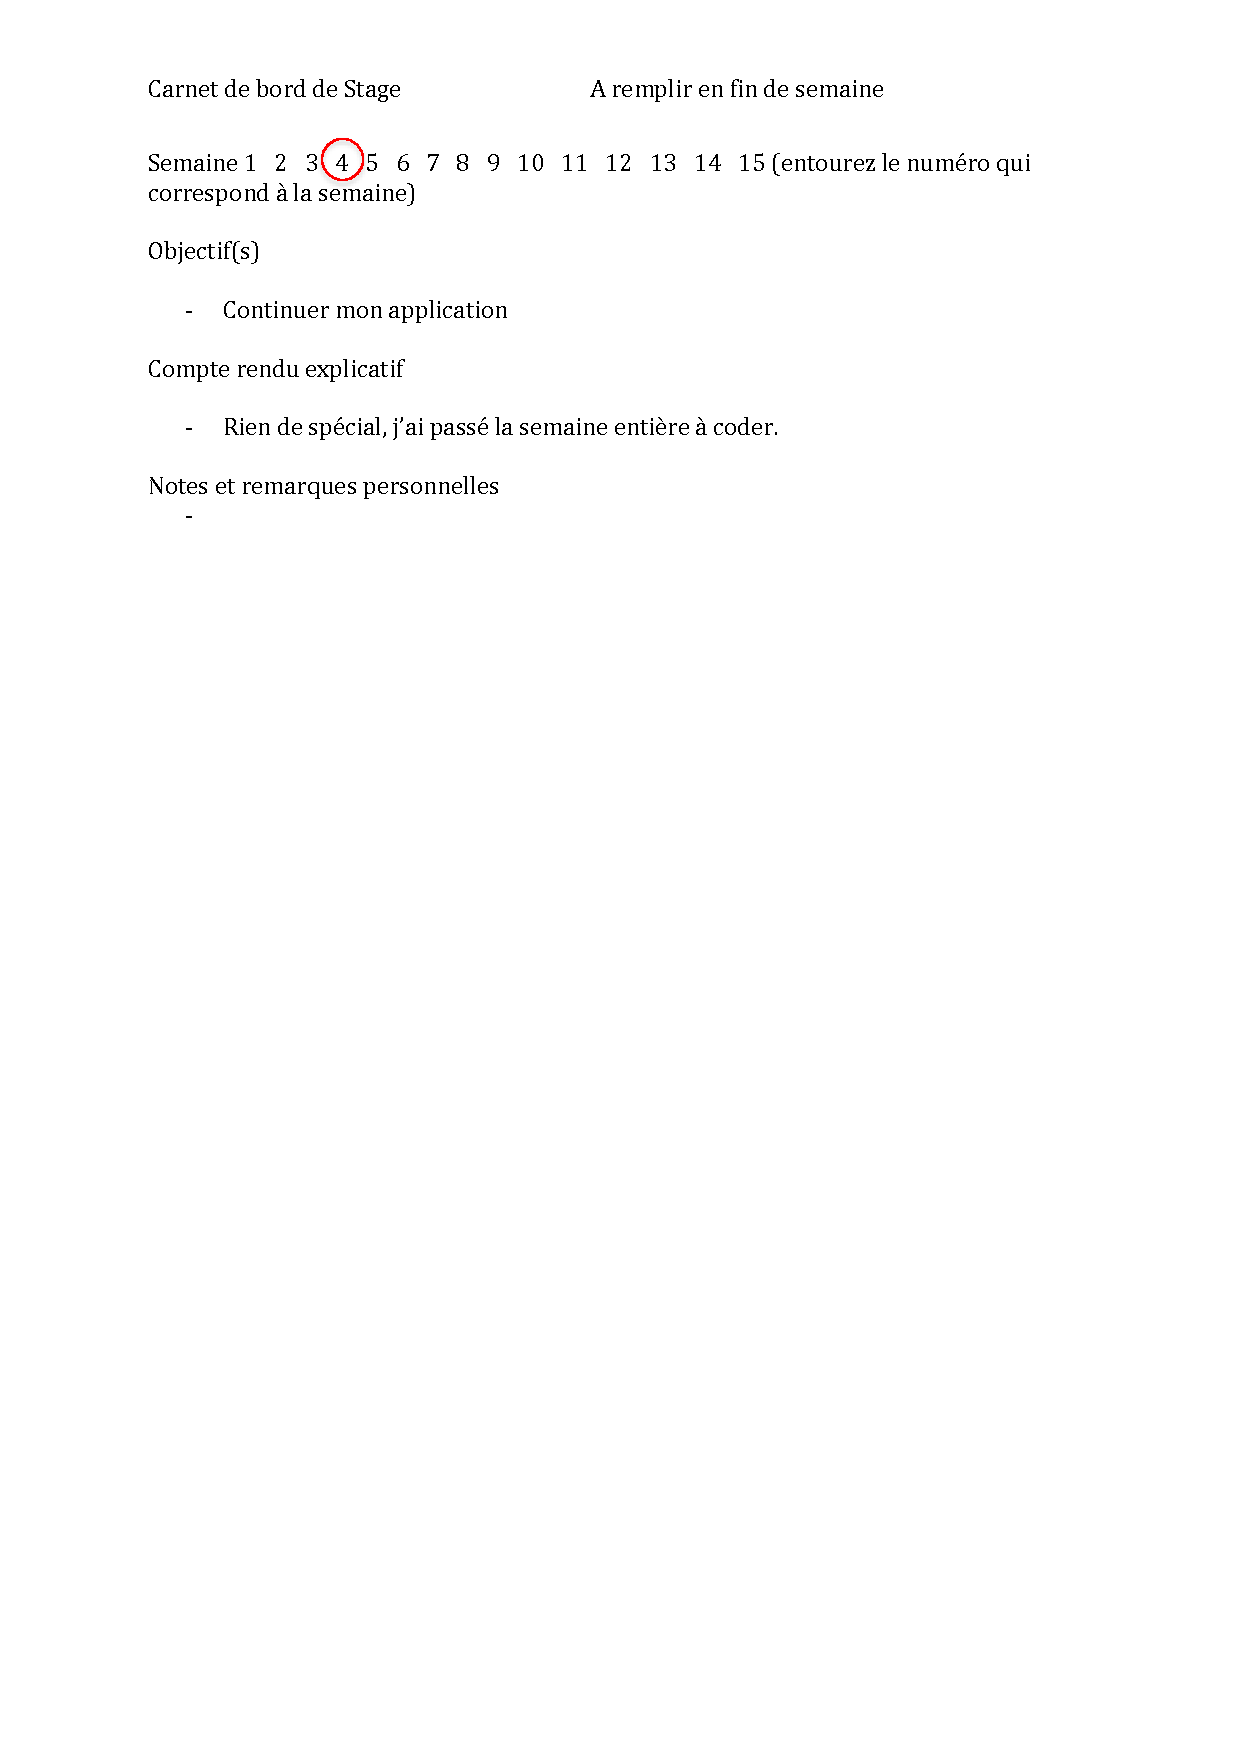
\includepdf[pages={1}]{carnets/Carnet_de_bord_de_Stage_S4.pdf}
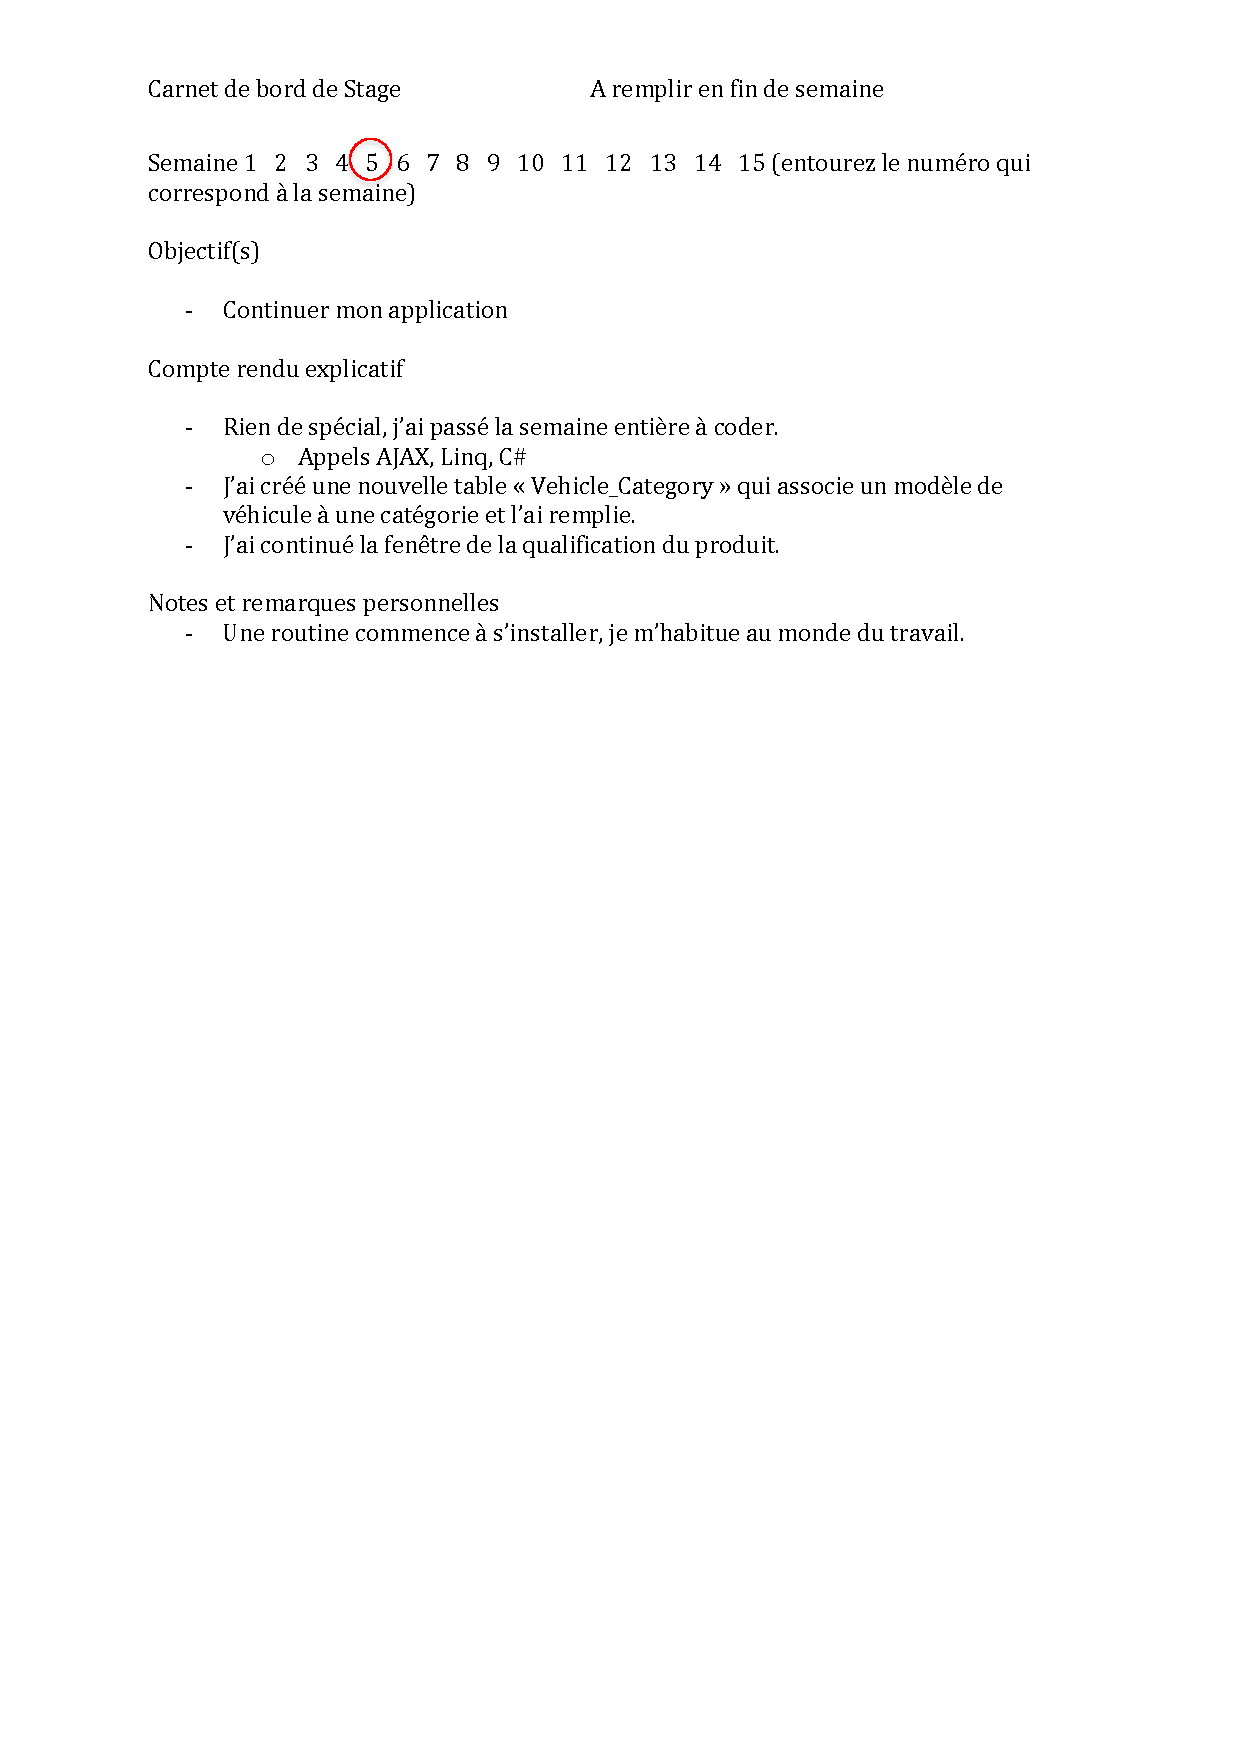
\includepdf[pages={1}]{carnets/Carnet_de_bord_de_Stage_S5.pdf}
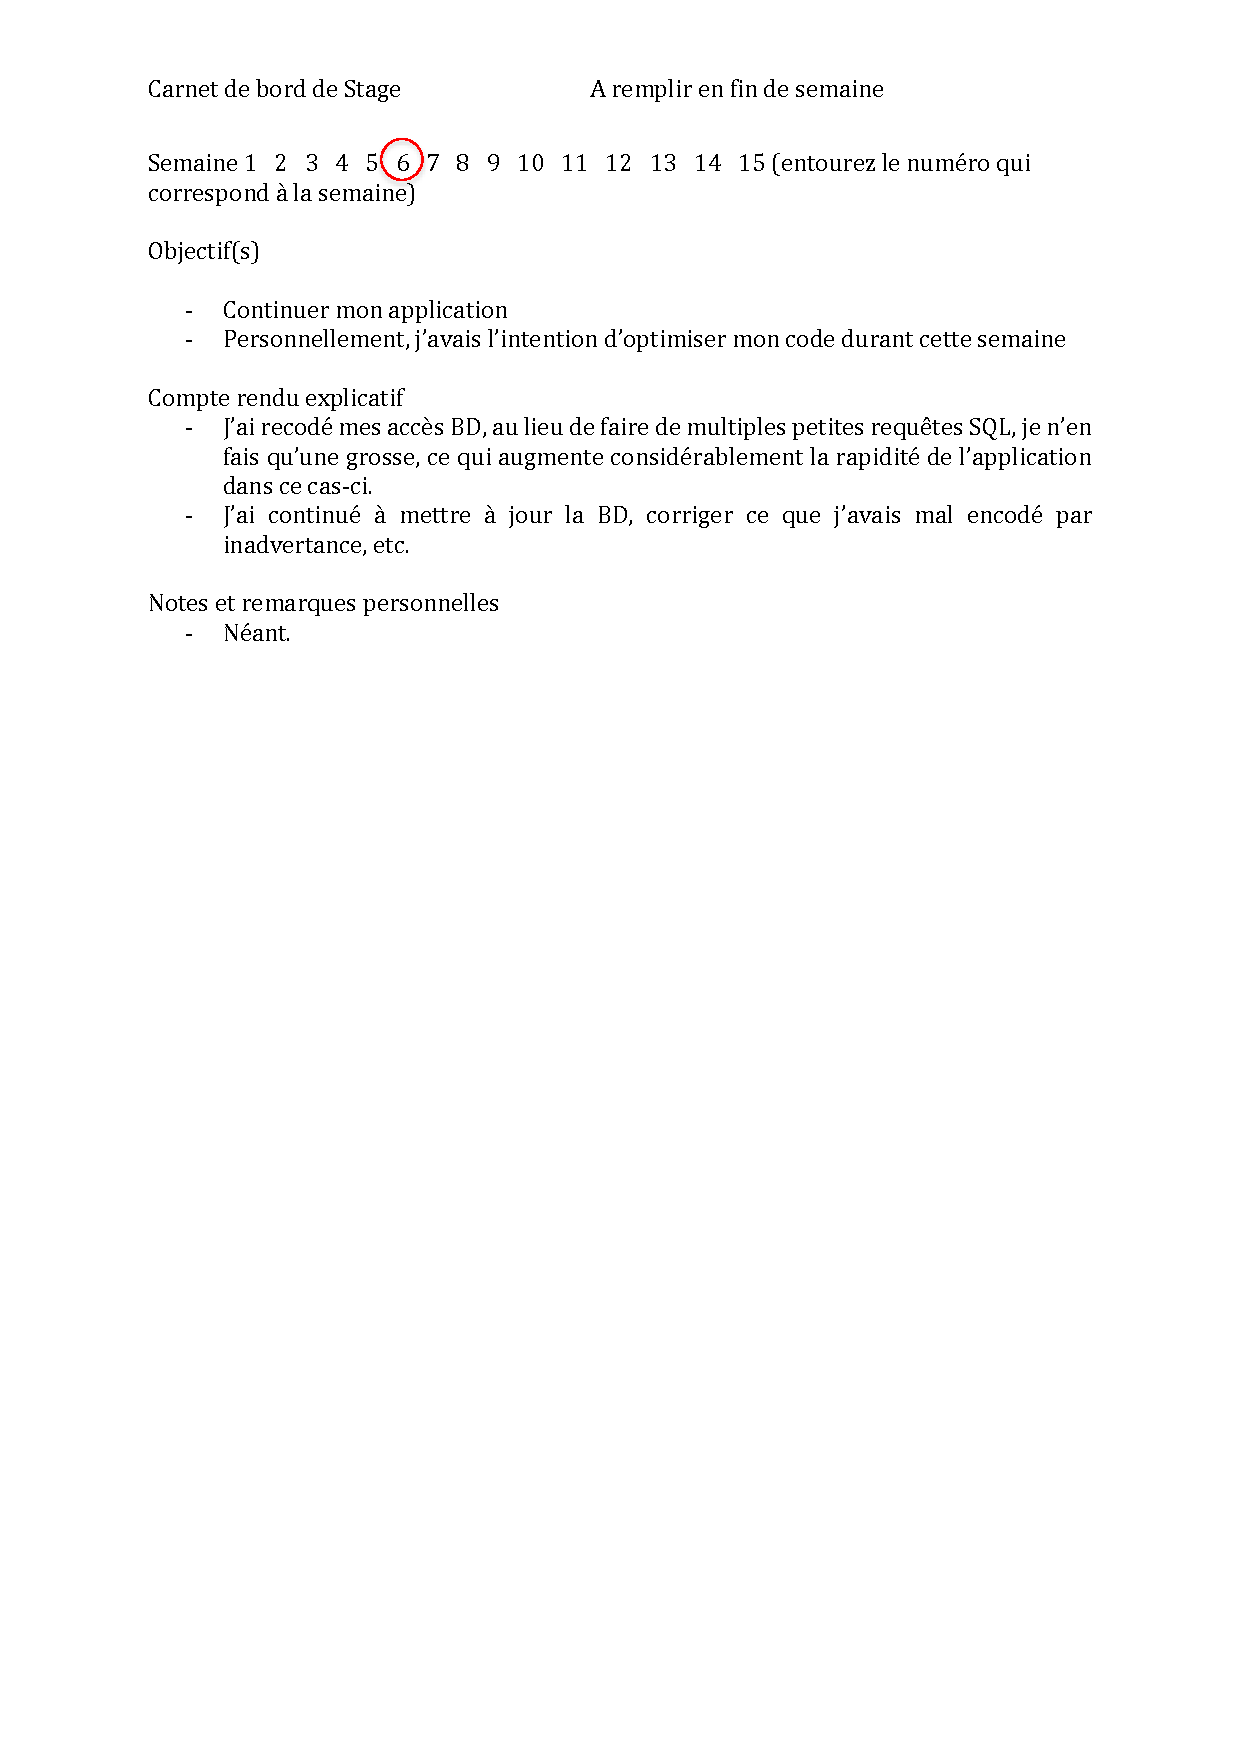
\includepdf[pages={1}]{carnets/Carnet_de_bord_de_Stage_S6.pdf}
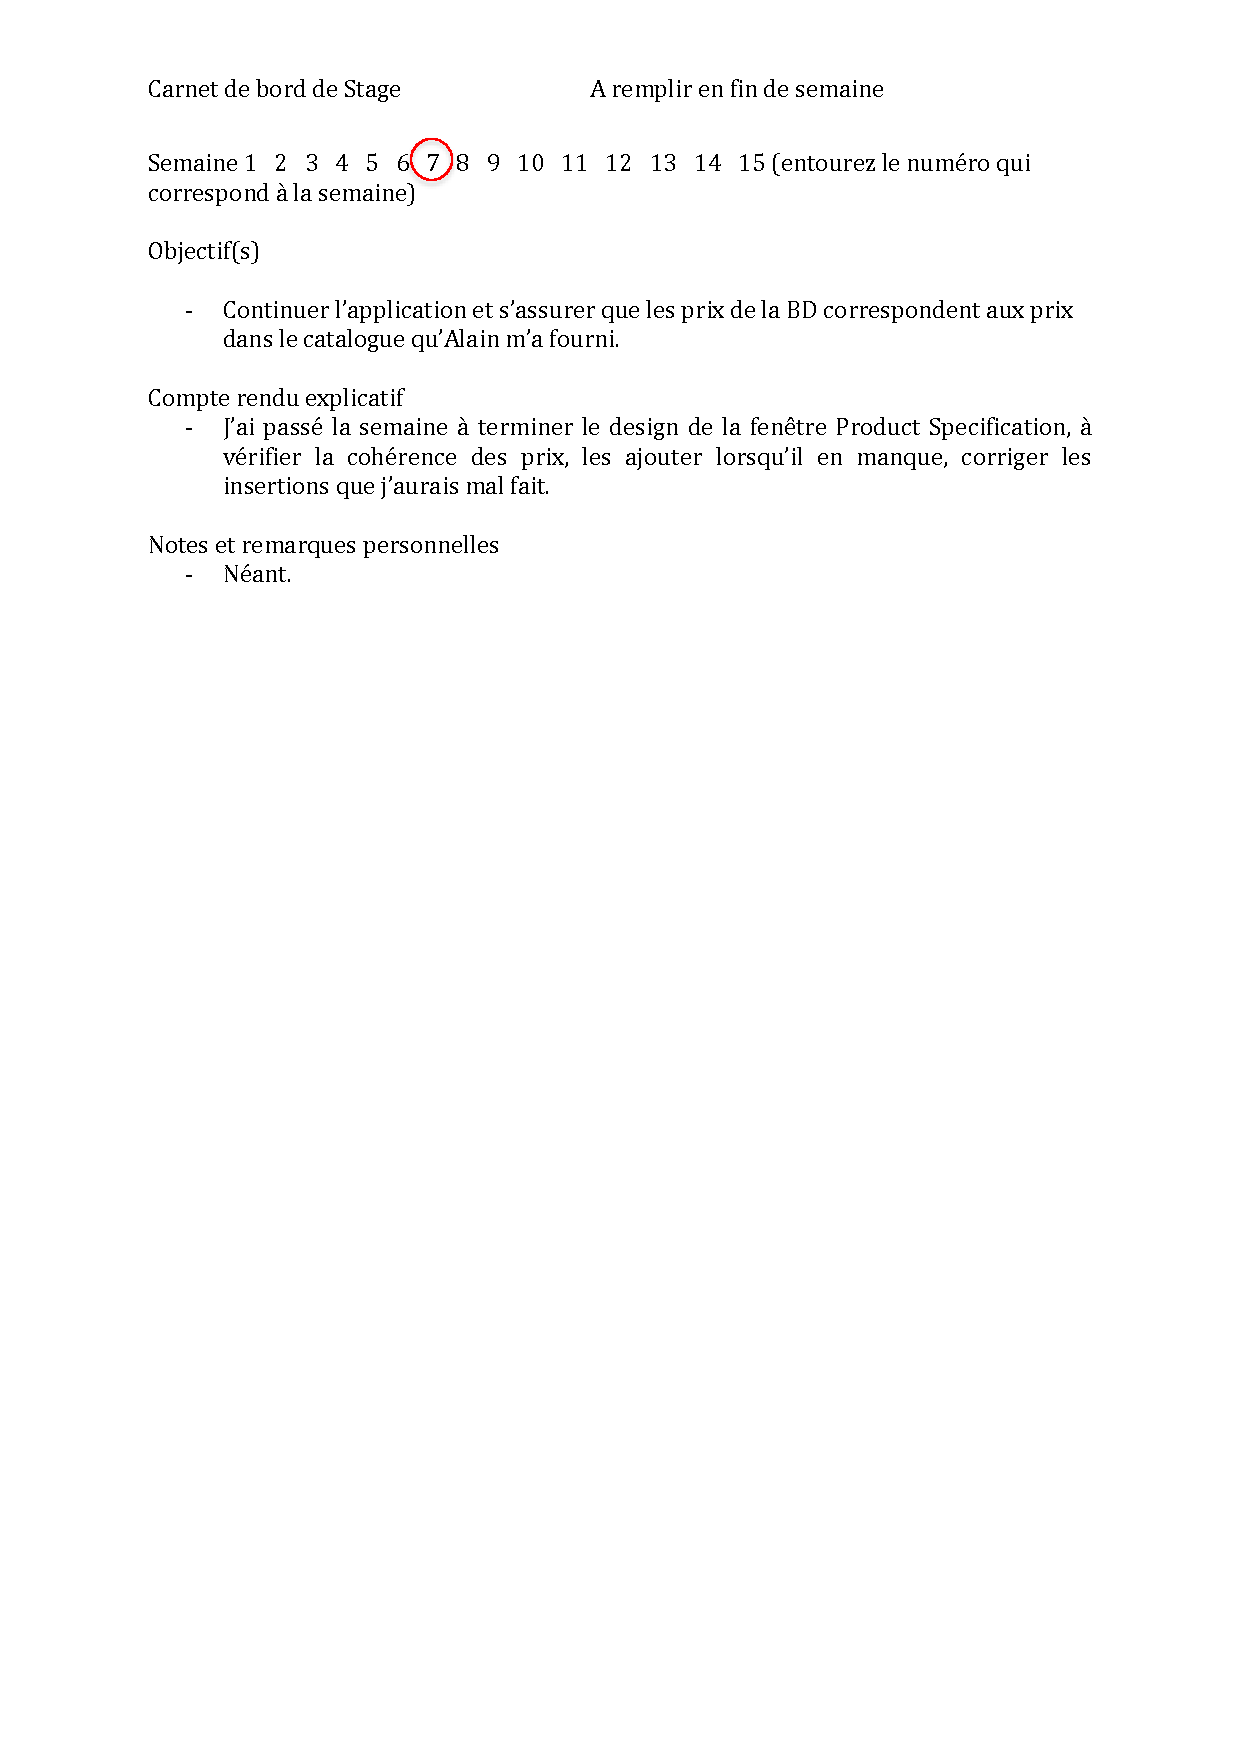
\includepdf[pages={1}]{carnets/Carnet_de_bord_de_Stage_S7.pdf}
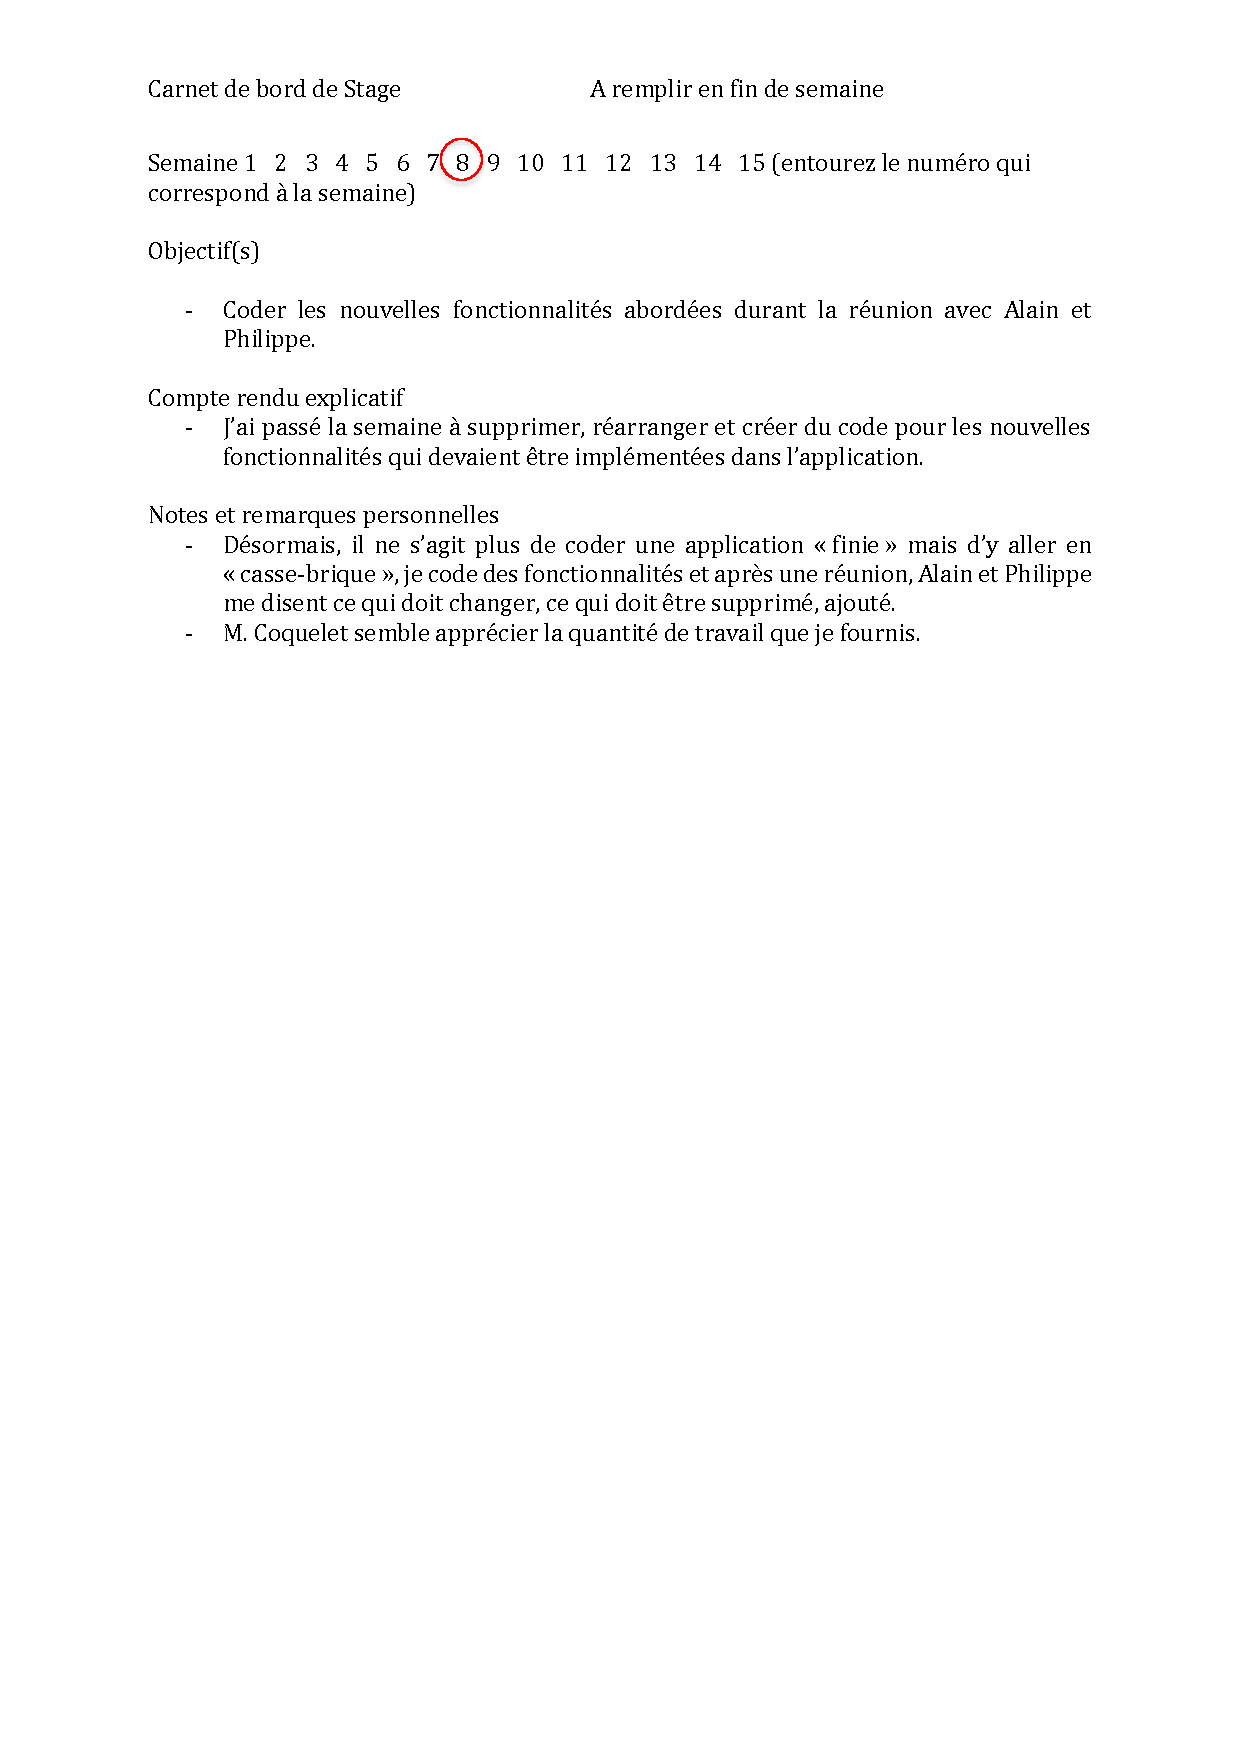
\includepdf[pages={1}]{carnets/Carnet_de_bord_de_Stage_S8.pdf}
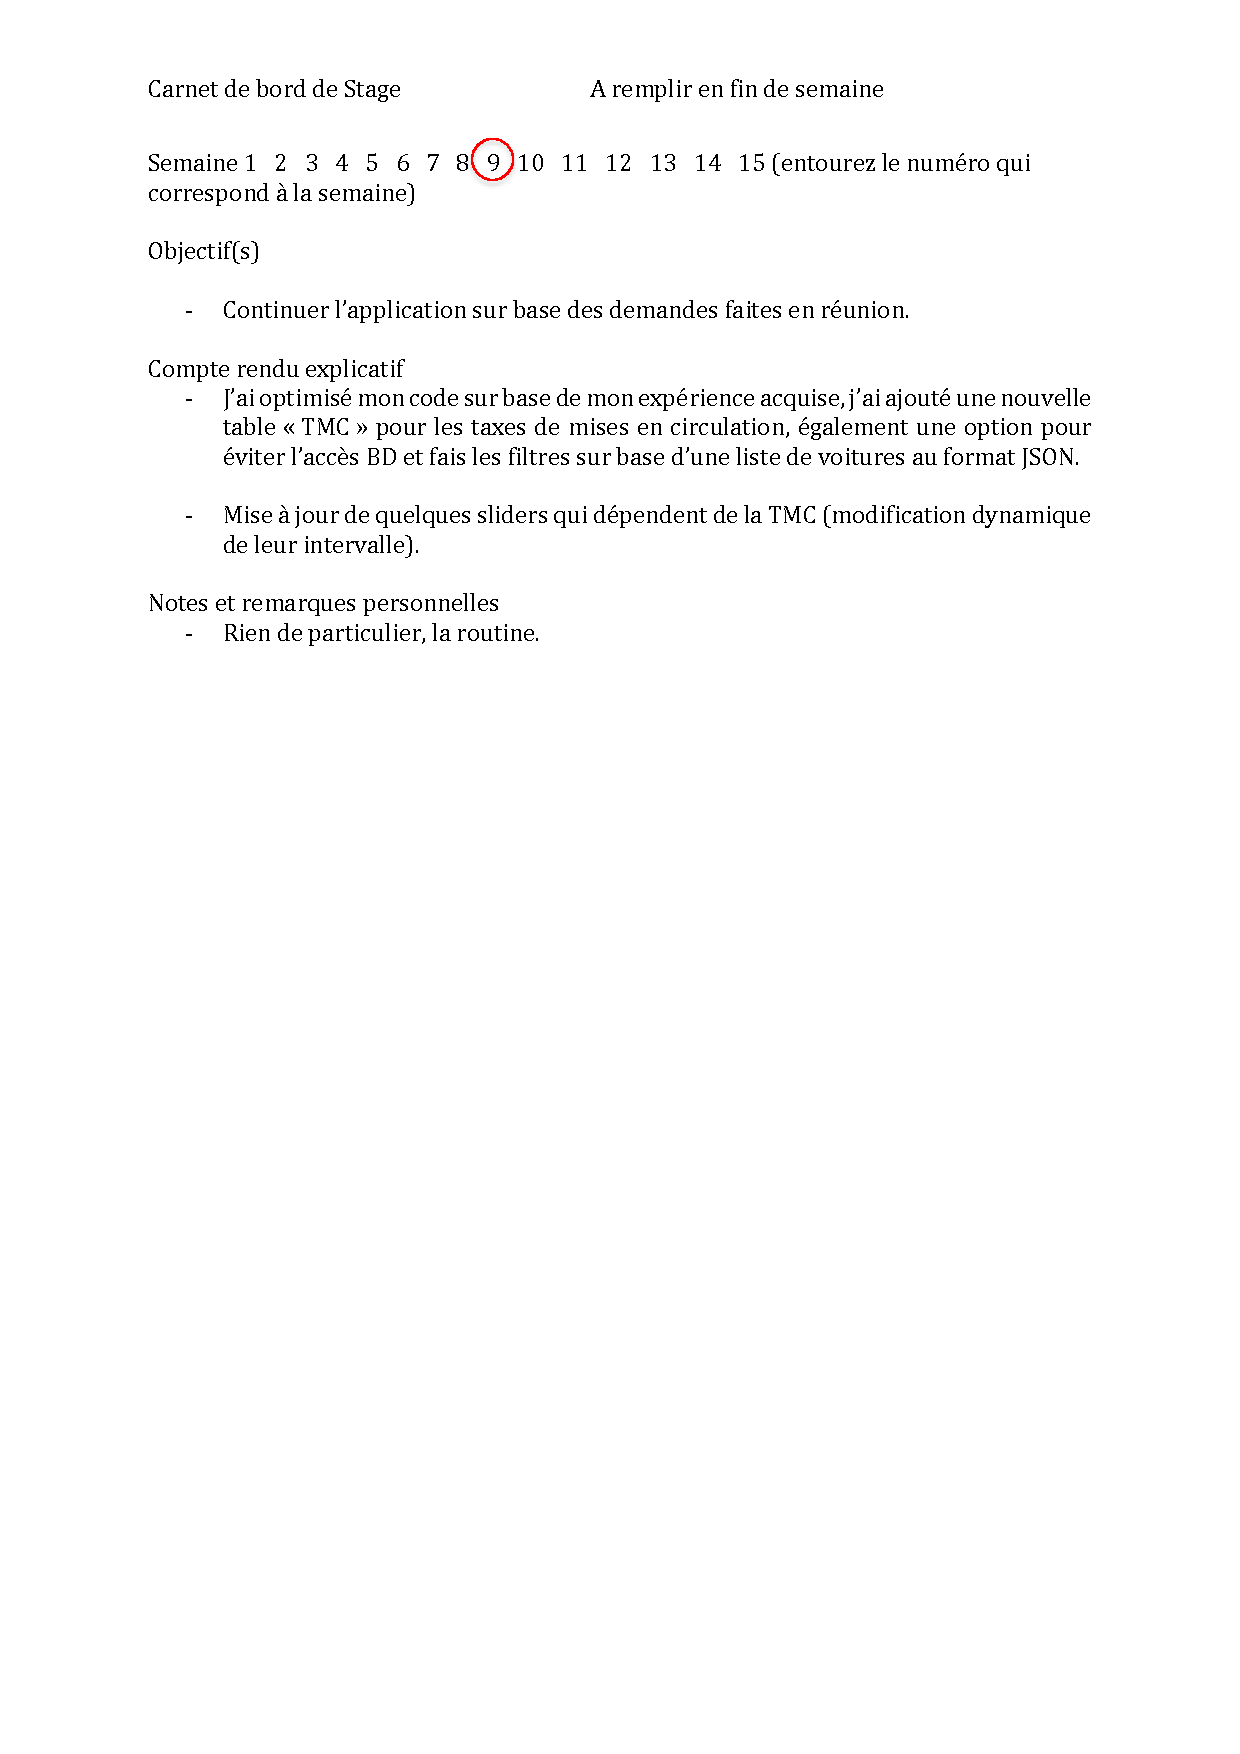
\includepdf[pages={1}]{carnets/Carnet_de_bord_de_Stage_S9.pdf}
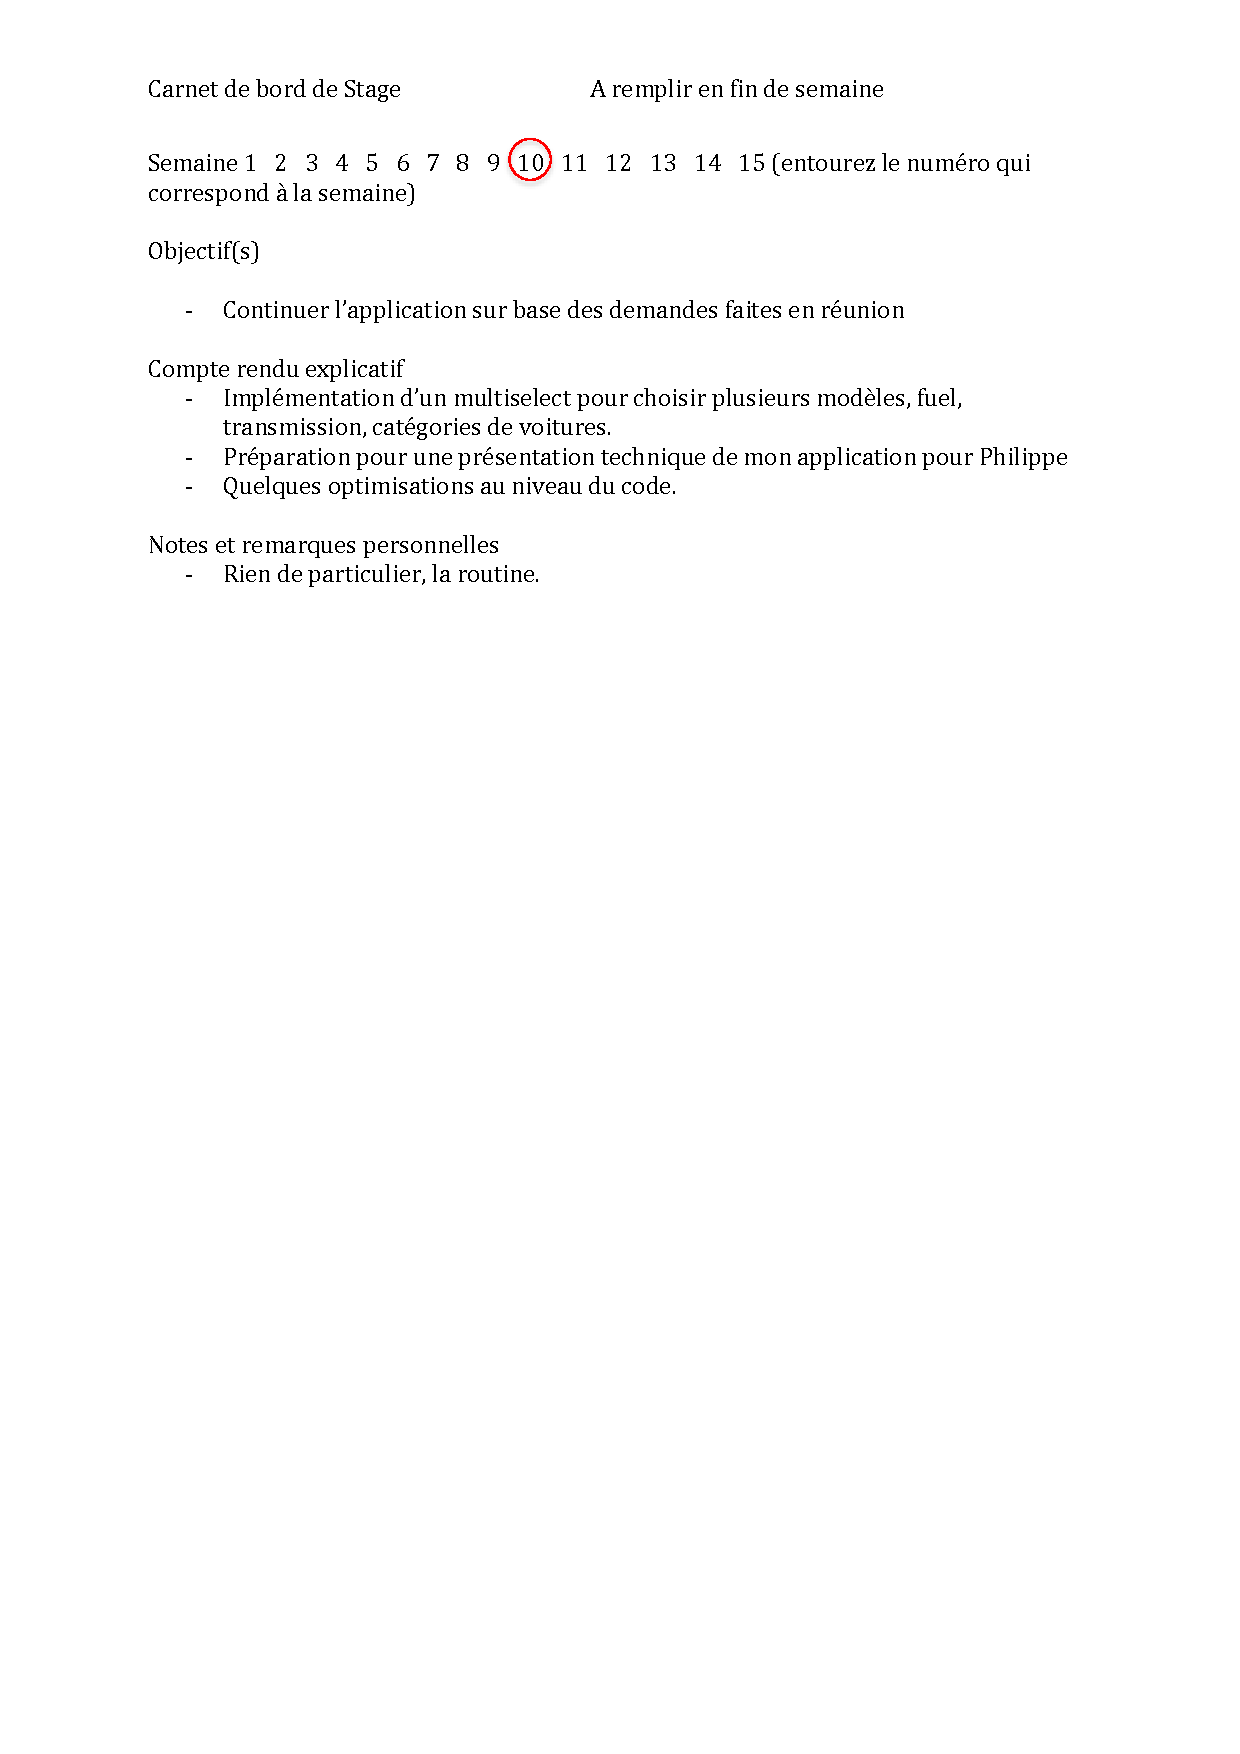
\includepdf[pages={1}]{carnets/Carnet_de_bord_de_Stage_S10.pdf}
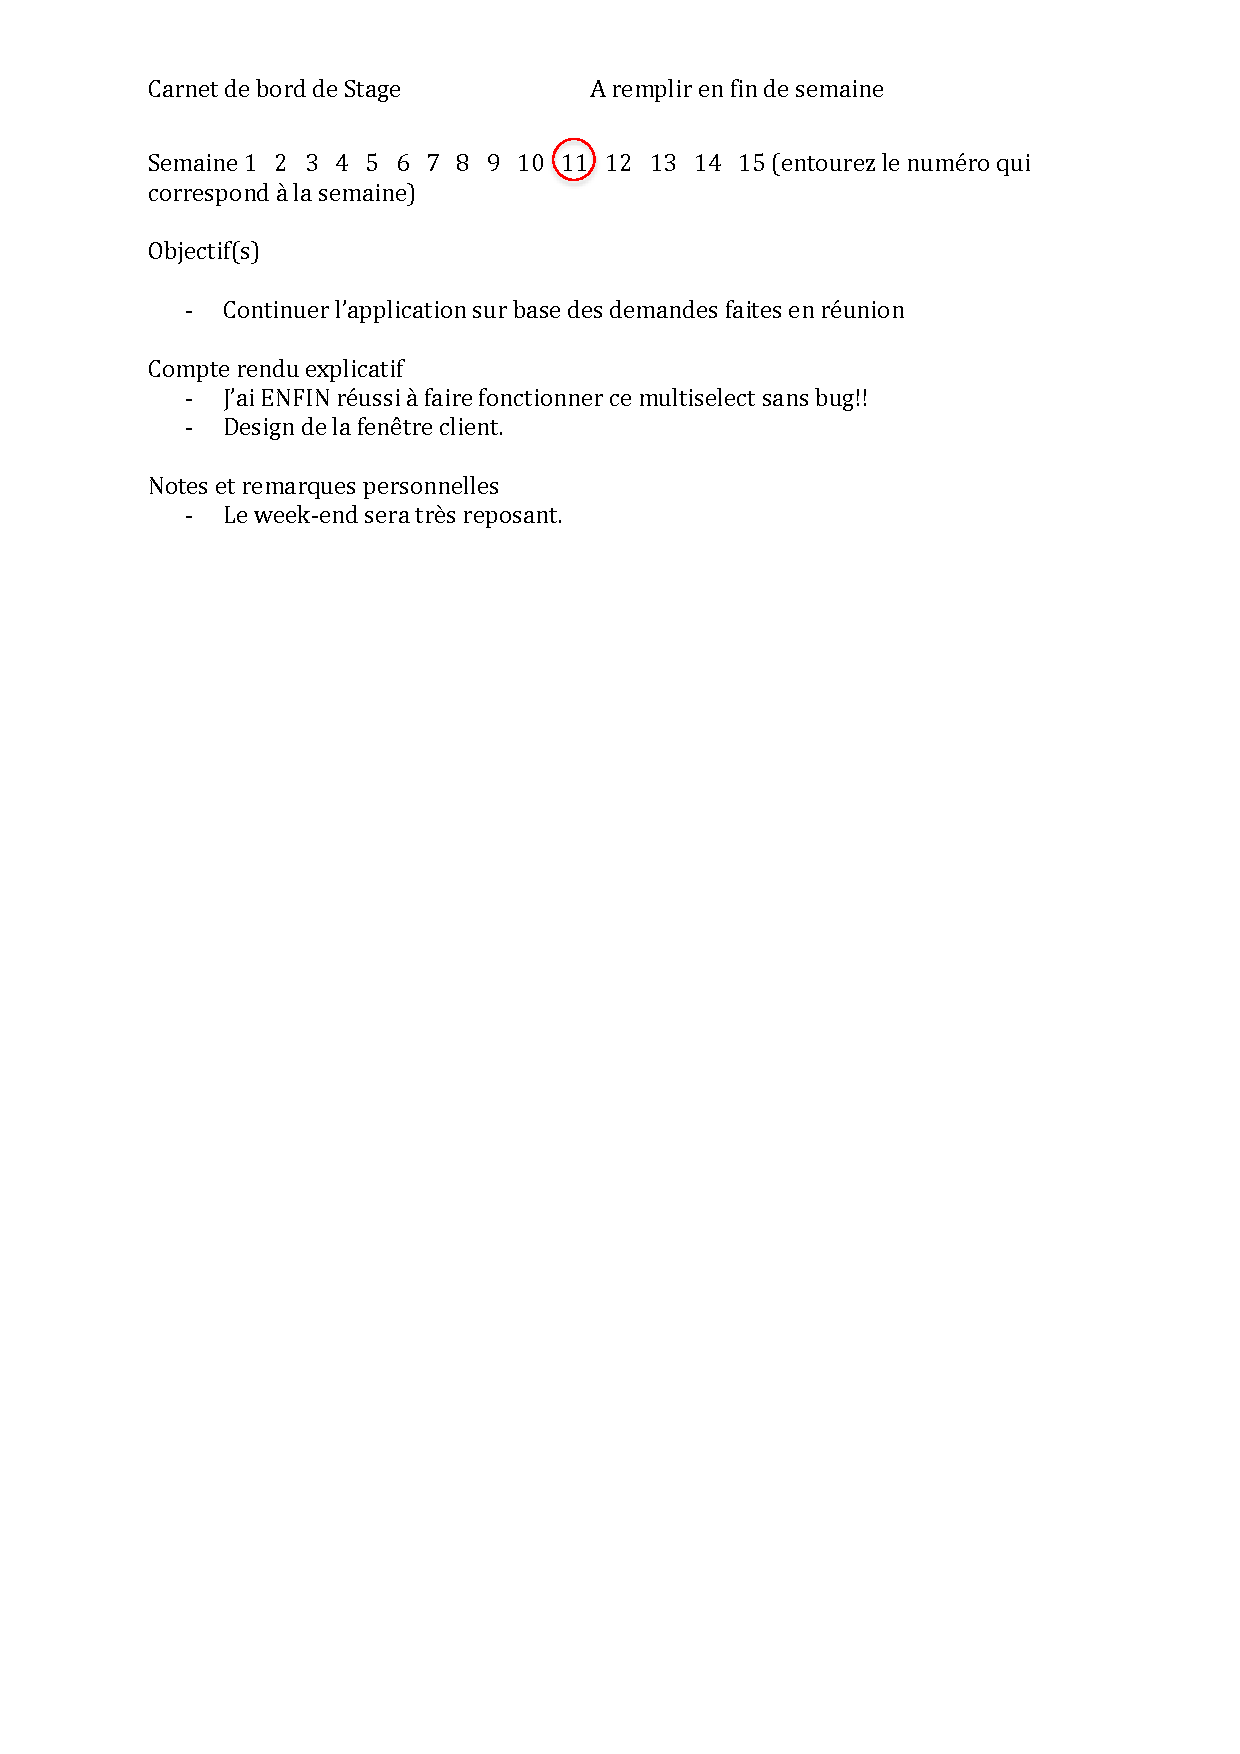
\includepdf[pages={1}]{carnets/Carnet_de_bord_de_Stage_S11.pdf}
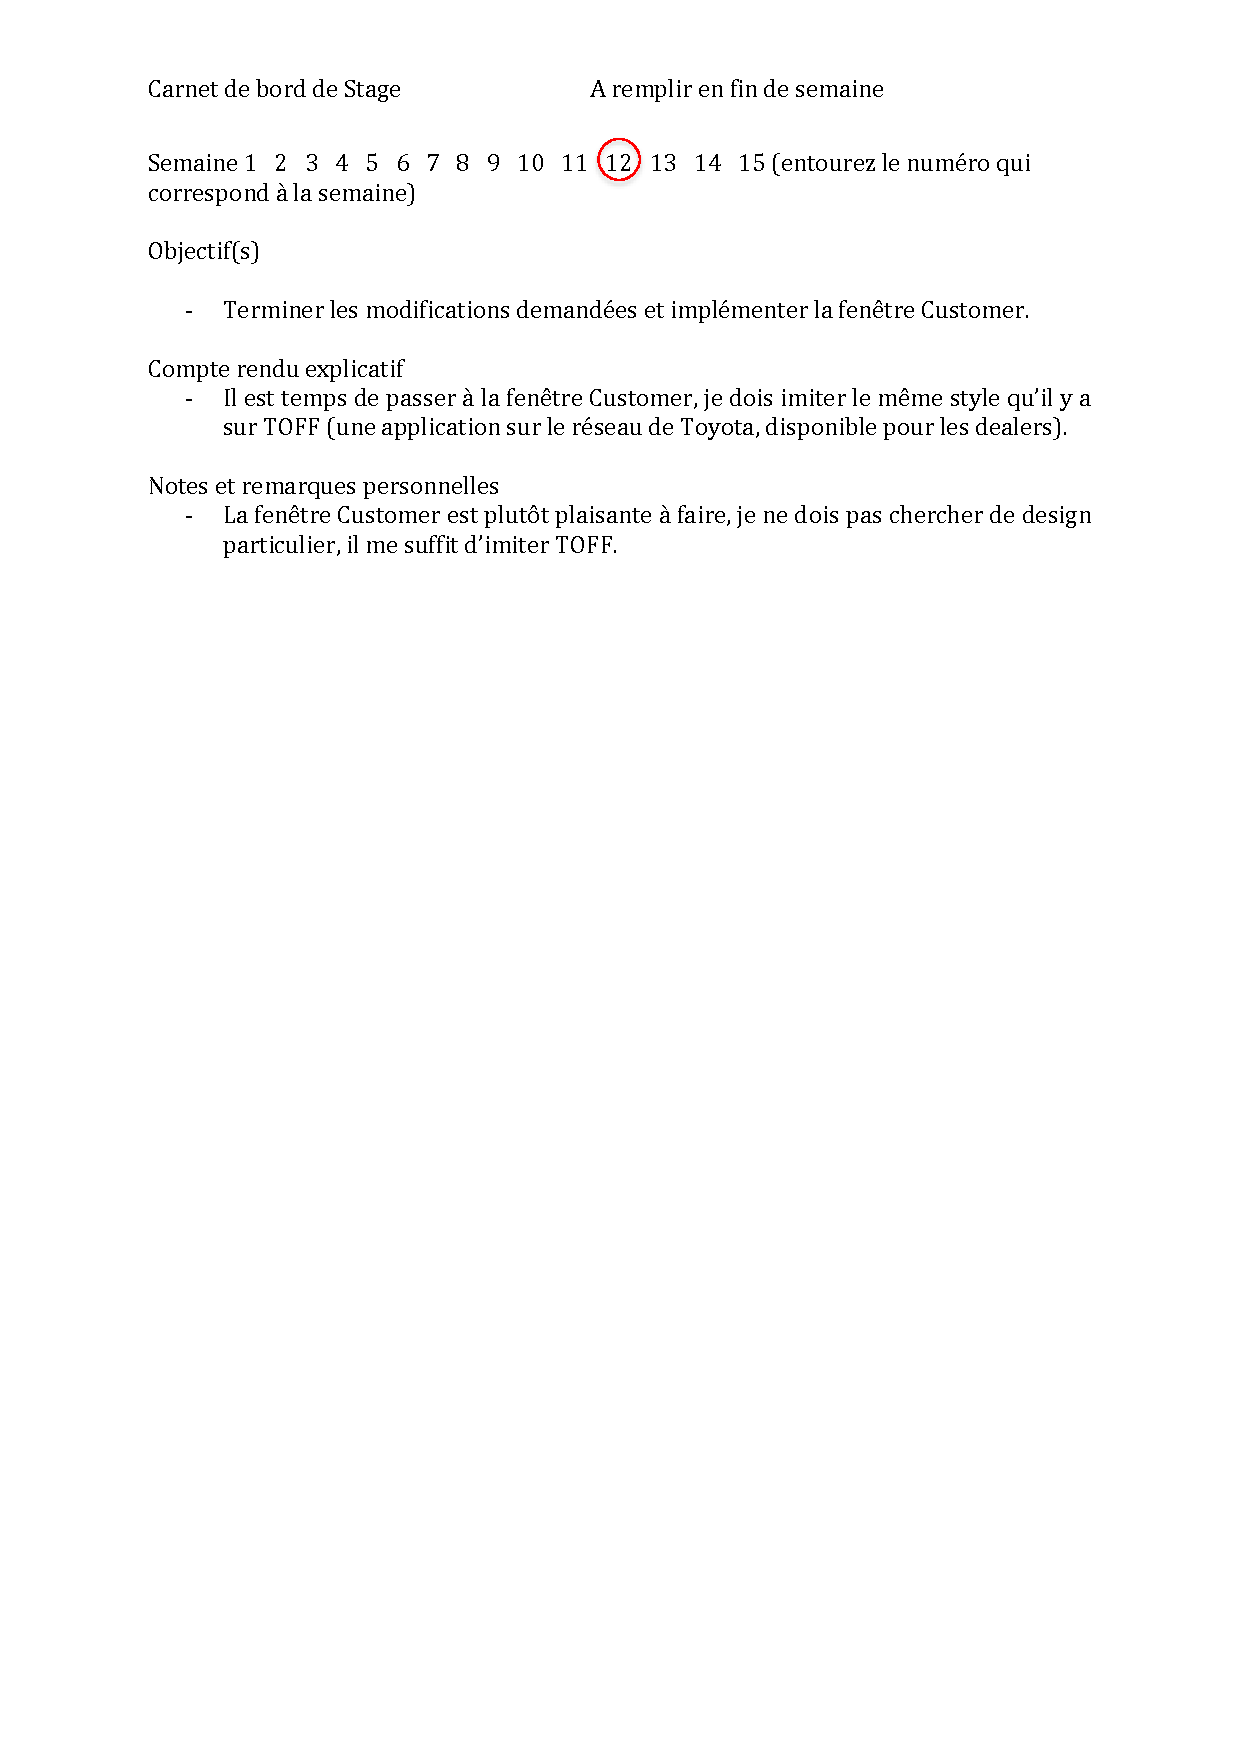
\includepdf[pages={1}]{carnets/Carnet_de_bord_de_Stage_S12.pdf}
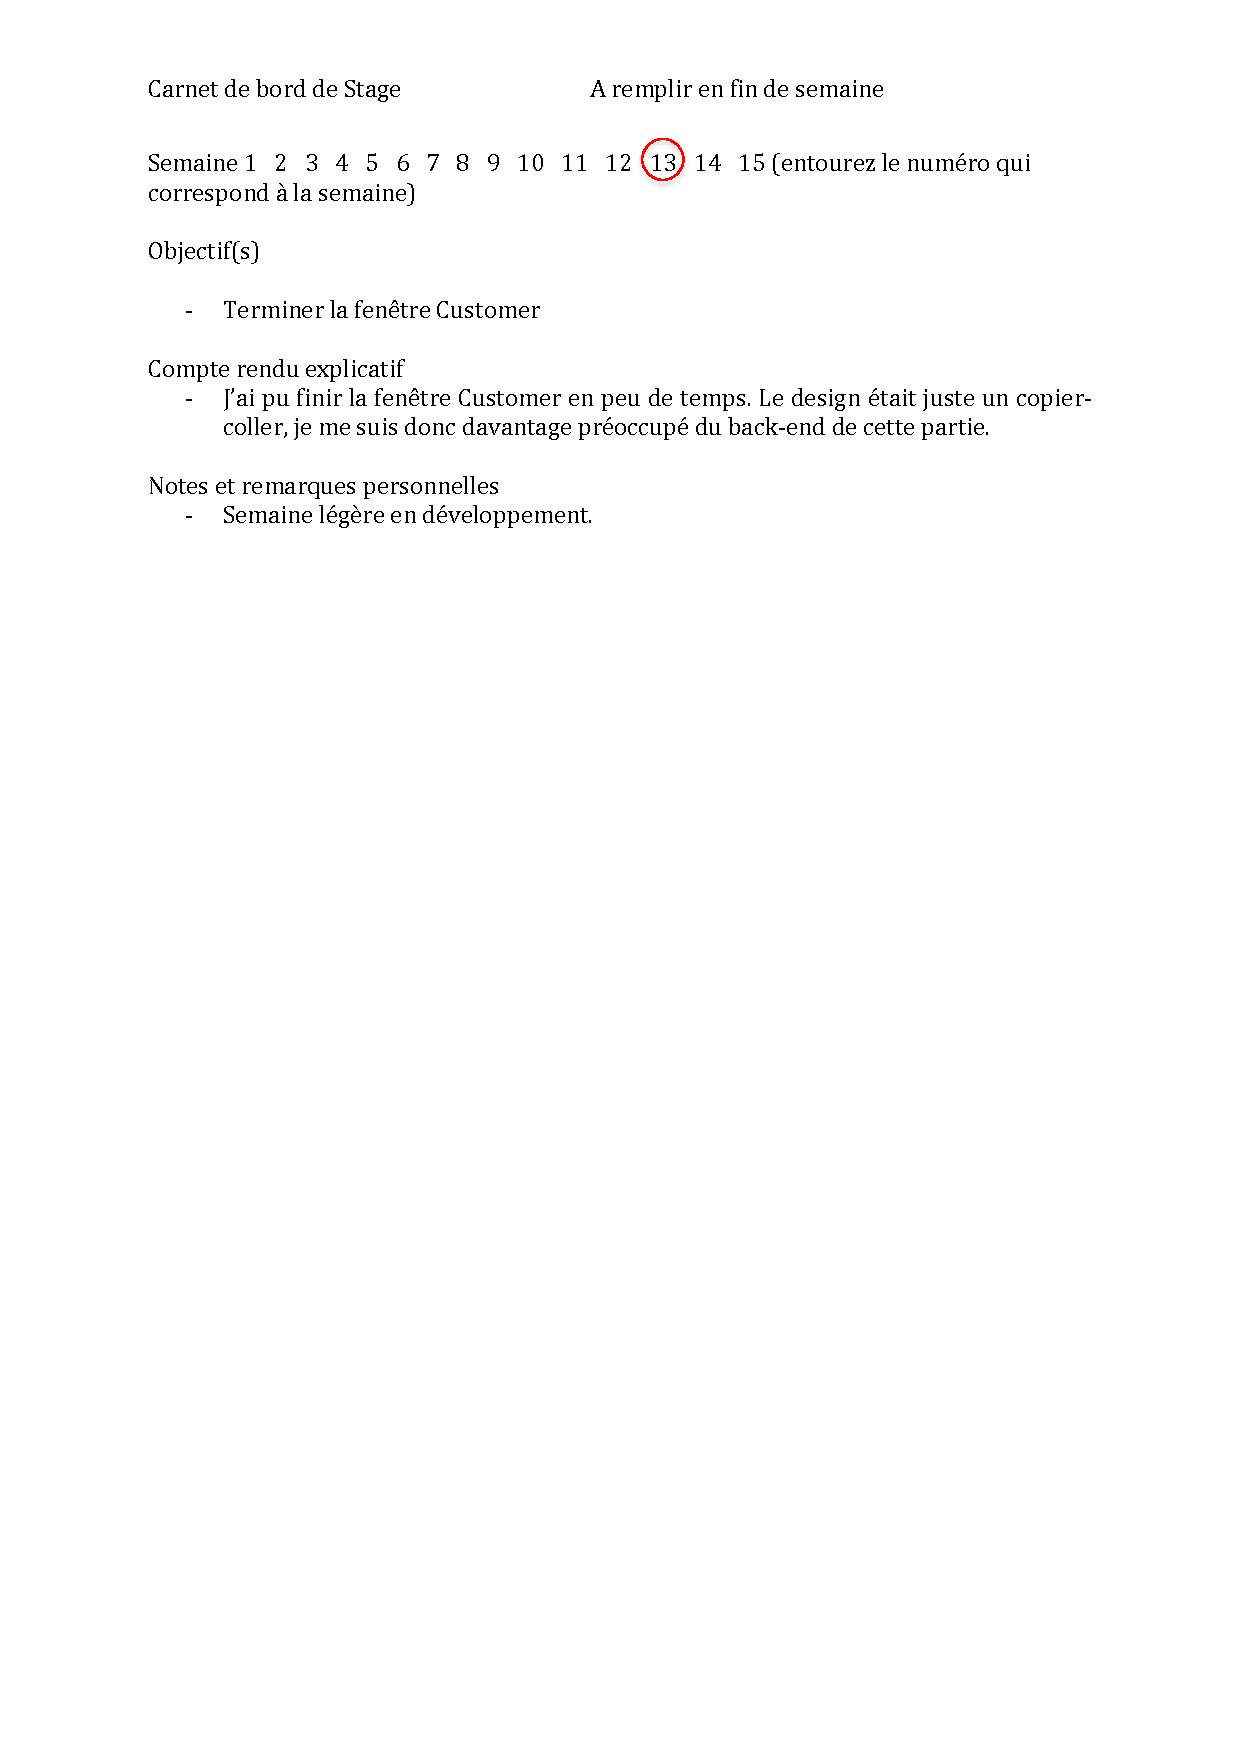
\includepdf[pages={1}]{carnets/Carnet_de_bord_de_Stage_S13.pdf}
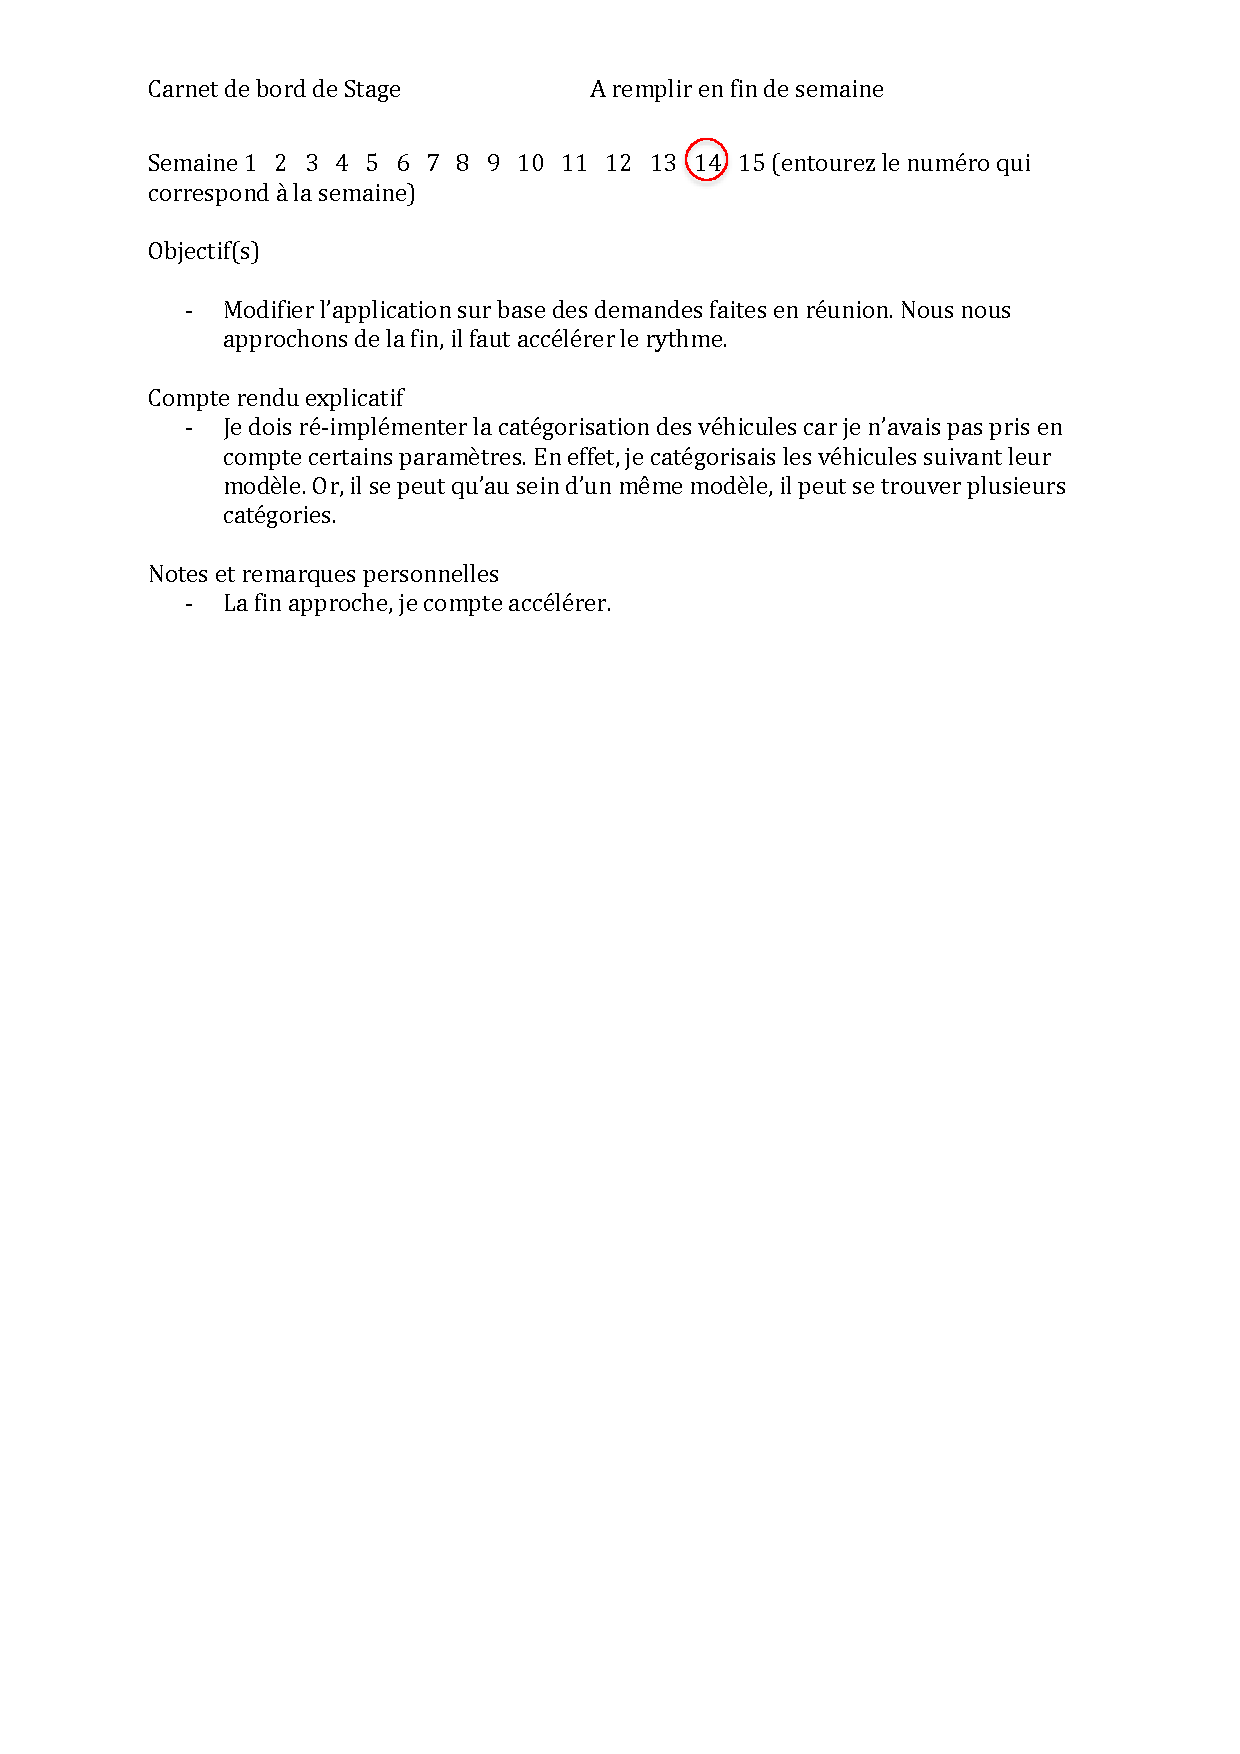
\includepdf[pages={1}]{carnets/Carnet_de_bord_de_Stage_S14.pdf}
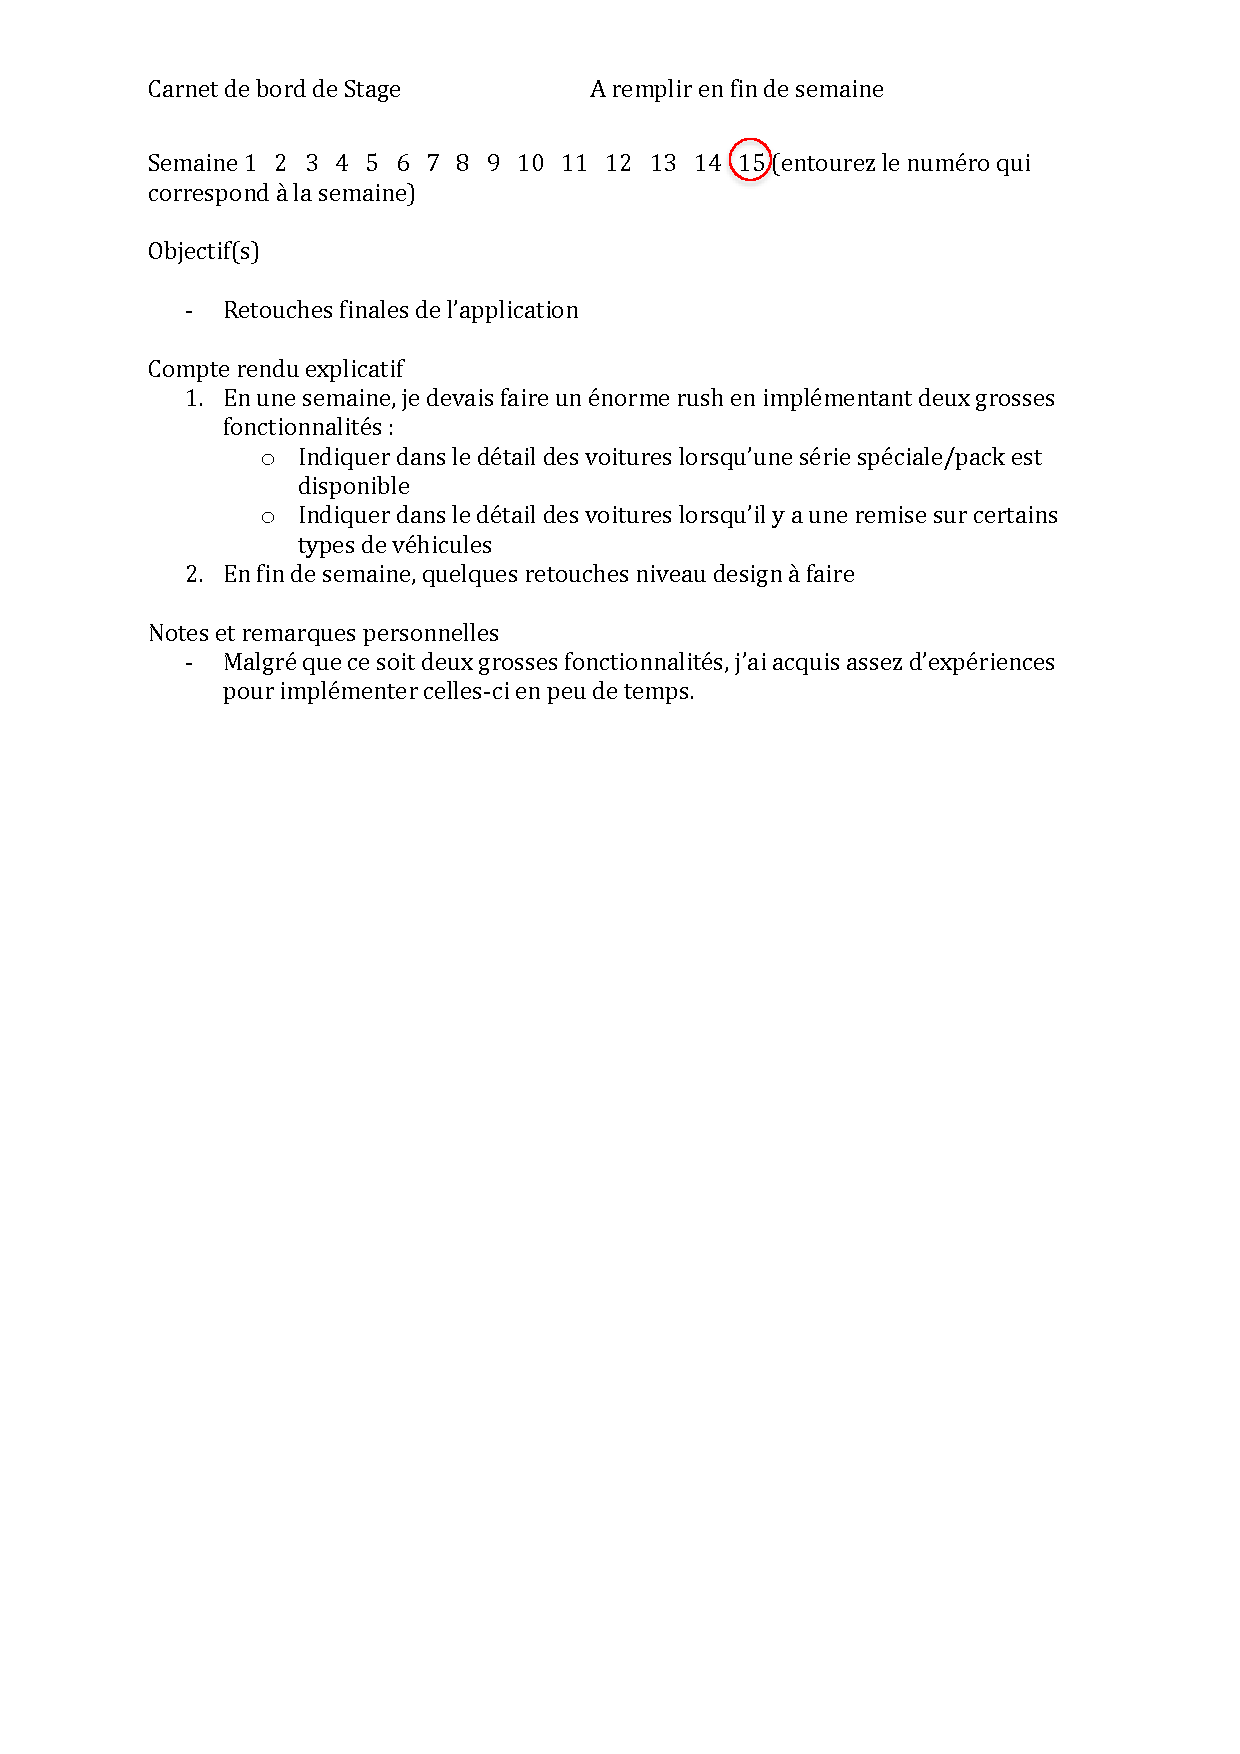
\includepdf[pages={1}]{carnets/Carnet_de_bord_de_Stage_S15.pdf}

\chapter{Évaluation du stage}
% En attente de la réponse de M. Coquelet

\chapter{Conclusion}
\paragraph{}
En conclusion, ce stage m'a énormément appris, j'ai passé un agréable moment au sein de TOYOTA Belgium et l'équipe est fort sympathique.
\paragraph{}
D'un point de vue technique, j'ai pu en apprendre énormément sur les technologies Microsoft (ASP .NET, C\#, Linq, etc.). J'ai aussi pu affiner mon expérience dans des technologies Web (librairie jQuery, jQuery UI, HTML5, CSS3, etc.).
\paragraph{}
Durant le stage, je me renseignais sur les dernières technologies Web, j'ai notamment pu apprendre à coder en SASS, à utiliser le framework BootStrap et découvert les medias queries en CSS. 
Malheureusement, comme le projet était déjà lancé lorsque j'apprenais ces nouvelles technologies durant mon temps libre, je ne pouvais plus les intégrer dans l'application car cela serait une trop grosse perte de temps.

\paragraph{}
Aussi, d'un point de vue organisationnel, j'ai appris à gérer mon emploi du temps de manière efficace. Tenir un planning de mes activités me paraît désormais beaucoup plus facile à faire qu'au début de mon stage. 

\paragraph{}
Enfin, j'ai appris que le plus important dans le métier d'informaticien n'est pas forcément de produire des milliers de lignes de code à la seconde. 
Il s'agit surtout d'apprendre à comprendre celui des autres et dès lors qu'on saura le faire, nous pourrons leur être bénéfiques.

% Bibliographie %
\addcontentsline{toc}{chapter}{Bibliographie} %Rajoute une entrée à la table des matière (toc)
\nocite{*}
\printbibliography
% Si aucune entrée n'est affichée, run pdftolatex puis bibtex puis pdftolatex 2x
\end{document}